\documentclass[a4paper,11pt,twoside]{article}

\usepackage{my-thesis-template}


%----------------------------------------------------------------------------------------
%	METADATA
%----------------------------------------------------------------------------------------
\newcommand{\thesistitle}{Robotic surgical tool manipulator - Recognition, control and manipulation of laparoscopic tools}
\newcommand{\division}{Division}
\newcommand{\me}{Karadimos Alexios of Loukas}
\newcommand{\nomme}{Karadimos Alexios of Loukas}
\newcommand{\studnum}{1046820}
\newcommand{\monthyear}{Month 2021}
\newcommand{\supname}{Evangelos Dermatas}
\newcommand{\suptitle}{Associate Professor Dr.}
\newcommand{\headofdivision}{Kazakos Demosthenes}
\newcommand{\headofdivisiontitle}{Assistant Professor Dr.}
\newcommand{\keywords}{surgery, robotics, control, laparoscopy}
\title{\thesistitle}
\author{Karadimos Alexios}
\date{2020}

% PDF metadata
\hypersetup
{
    pdfauthor={Alexios Karadimos},
    pdftitle={thesis},
    pdfsubject={\thesistitle},
    pdfkeywords={\keywords},
    pdfproducer={PdfLaTex},
    pdfcreator={Alexios Karadimos}
}



\begin{document}

\selectlanguage{greek}
\selectlanguage{english}


%----------------------------------------------------------------------------------------
%	FRONT PAGE & CERTIFICATION
%----------------------------------------------------------------------------------------
\begin{titlepage}
\begin{center}
% Upper part of the page
\textsc{\textbf{\large UNIVERSITY OF PATRAS - SCHOOL OF ENGINEERING}\\
\large DEPARTMENT OF ELECTRICAL AND COMPUTER ENGINEERING}\\


\includegraphics[width= 0.5\textwidth]{up_2017_logo_gr.png}\\  

\textsc{Division: \large Systems and Automatic Control}\\[1cm]

\textsc{\textbf{\LARGE{Thesis}}}\\ [0.5cm]
of the student of the Department of Electrical and Computer Engineering of the School of Engineering of the University of Patras\\[0.5cm]

\textsc{\Large \me }\\[0.5cm]
\textsc{\large Student Number: 1046820}\\[1cm]

\underline{\large Subject}\\
\HRule \\[0.4cm]
{\huge \bfseries \thesistitle }\\[0.4cm] % Title of your document
\HRule \\[1.5cm]

\underline{\large Supervisor}\\[0.5cm]
\large \suptitle \, \supname \\[1cm]
\textbf{Thesis Number:}
%\large 1046820/2020
\vfill
% Bottom of the page
\large{Patras, 2020}
\end{center}
\end{titlepage}

% \begin{titlepage}

% %----------------------------------------------------------------------------------------
% %	HEADING SECTIONS
% %----------------------------------------------------------------------------------------

% \Large UNIVERSITY OF PATRAS - SCHOOL OF ENGINEERING\\[0.5cm] % Name of your university/college
% \textsc{\Large DEPARTMENT OF ELECTRICAL AND COMPUTER ENGINEERING}\\[0.5cm] % Major heading such as course name
% \textsc{\large \textlatin{ECE}ΔΚ803}\\[0.5cm] % Minor heading such as course title

% %----------------------------------------------------------------------------------------
% %	TITLE SECTION
% %----------------------------------------------------------------------------------------


% %----------------------------------------------------------------------------------------
% %	AUTHOR SECTION
% %----------------------------------------------------------------------------------------


% % If you don't want a supervisor, uncomment the two lines below and remove the section above
% %\Large \emph{Author:}\\
% \emph{Αλέξιος Καραδήμος}\\ % Your name
% Τμήμα Ηλεκτρολόγων Μηχανικών \& Τεχνολογίας Υπολογιστών\\[2cm]

% %----------------------------------------------------------------------------------------
% %	DATE SECTION
% %----------------------------------------------------------------------------------------

% {\large 2020}\\[1cm] % Date, change the \today to a set date if you want to be precise

% %----------------------------------------------------------------------------------------
% %	LOGO SECTION
% %----------------------------------------------------------------------------------------

% \begin{center}
% 
\includegraphics[width=5cm]{images/up_2017_logo_gr.png}\\[1cm] % Include a department/university logo - this will require the graphicx package
% \end{center}

% %----------------------------------------------------------------------------------------

% \vfill % Fill the rest of the page with whitespace

% \end{titlepage}

\pagestyle{empty}
\begin{center}
{\LARGE \textbf{ΠΙΣΤΟΠΟΙΗΣΗ}\\[1cm]}
\large Πιστοποιείται ότι η διπλωματική εργασία με θέμα\\[1cm]
\textbf{\large \thesistitle }\\[1cm]
του φοιτητή του Τμήματος Ηλεκτρολόγων Μηχανικών και Τεχνολογίας Υπολογιστών\\[1.5cm]
\me \\[0.5cm]
(Α.Μ.: \studnum )\\[1.5cm]
παρουσιάστηκε δημόσια και εξετάστηκε στο τμήμα  Ηλεκτρολόγων Μηχανικών και Τεχνολογίας Υπολογιστών στις\\[1cm]
\Large{\_\_/\_\_/\_\_\_}\\[1.5cm]
\end{center}
\begin{minipage}{0.5\textwidth}
\begin{flushleft} \large
Ο Επιβλέπων\\[4cm]
\supname \\
\emph{\suptitle}
\end{flushleft}
\end{minipage}
\begin{minipage}{0.5\textwidth}
\begin{flushright} \large
Ο Διευθυντής του Τομέα\\[4cm]
\headofdivision\\
\emph{\headofdivisiontitle}
\end{flushright}
\end{minipage}

\newpage{\pagestyle{empty}\cleardoublepage}
\newpage
\pagestyle{empty}
\begin{center}
{\LARGE \textbf{CERTIFICATION}\\[1cm]}
\large It is certified that the Thesis with Subject\\[1cm]
\textbf{\large \thesistitle }\\[1cm]
of the student of the Department of Electrical and Computer Engineering\\[1.5cm]
\me \\[0.5cm]
(R.N.: \studnum )\\[1.5cm]
Was presented publicly and defended at the Department of Electrical and Computer Engineering at\\[1cm]
\Large{\_\_/\_\_/\_\_\_}\\[1.5cm]
\end{center}
\begin{minipage}{0.5\textwidth}
\begin{flushleft} \large
The supervisor\\[4cm]
\supname \\
\emph{\suptitle}
\end{flushleft}
\end{minipage}
\begin{minipage}{0.5\textwidth}
\begin{flushright} \large
The Director of the Division\\[4cm]
\headofdivision\\
\emph{\headofdivisiontitle}
\end{flushright}
\end{minipage}


%----------------------------------------------------------------------------------------
%	TABLE OF CONTENTS
%----------------------------------------------------------------------------------------

\pagestyle{fancy}

\clearpage
\tableofcontents
\renewcommand*\contentsname{Table of Contents}

%----------------------------------------------------------------------------------------
%	MAIN SECTIONS
%----------------------------------------------------------------------------------------

\newpage
\section{Introduction}

\subsection{Surgery Robotics}

Surgery Robotics is a field of Surgery where the surgeon operaties on the patient via a computer, specialised equipment and robotic arms, 
to which the surgical tools needed for the operation are attached. According to surgical bibliography, robotics and laparoscopic procedures are used 
in general surgery, cardiothoracic surgeries, colon surgeries, gynecology, neurosurgery and orthopedics. \\

Robotic mechanisms were first introduced in Medicine, in 1987 with the first laparoscopic surgery of a cholecystectomy. Since then numerous laparoscopic 
operations have been performed and there has been a lot of improvements and innovations in this field. Such surgical operations are characterised as 
\textbf{minimally invasive}, because the surgical incisions made at the patient are very small and thus the probability of infection of the patient during 
or after the operation are very small, the hospitalization time is reduced (which means mean better and more efficient use of hospital resources) and the overall 
recovery of the patient is significantly faster and less painful. \\

However, traditional laparoscopic mechanisms have some downsides as well. First of all, the surgeon should operate in a mirrored-way, meaning that they should 
move at the opposite direction from what they saw at the screen (this effect is also known as the \textbf{fulcrum effect}), in order to reach the desired point of operation. Earlier laparoscopic tools had less 
degrees of freedom, which means less flexibility in motion control. Moreover these systems provided limited touch sensibility and feedback to the doctor they 
were very susceptible to the surgeon's micro movements and tremble. \\

The first application of robotics in Surgery appears in 1985, when Kwoh et al. \cite{Shao1985ANC} used a \textbf{PUMA 560}, a standard industrial robotic arm, to perform a neurosurgical biopsy, 
where the biopsy needle was inserted in the brain and guided with the help of Computed Tomography. This successful application was followed by the \textbf{PROBOT} surgical robot \cite{Probot1992}, 
which was developed at the Imperial College and used in a prostatectomy operation. Another example of an early surgery robot was the \textbf{ROBODOC} system \cite{Robodoc} developed by Integrated Surgical Supplies 
in Sacramento California, which was the first to be used in orthopedics for a hip replacement surgery and was also the first to be approved by the FDA (Food \& Drug Administration, organization responsible 
for medical devices, drugs etc.).

\begin{center}
\begin{figure}[H]
\centering
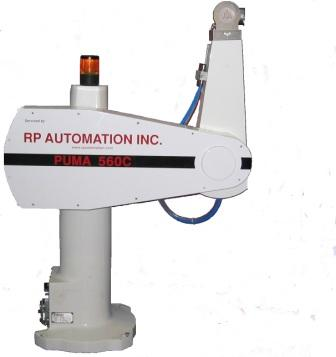
\includegraphics{images/Puma560.jpg}\\
\caption{The PUMA 560 robotic arm, which was the first to be used in surgery robotics in 1985}
\end{figure}
\end{center}

Some other important surgery robots are listed below:
\begin{itemize}
\item \textbf{AESOP\textsuperscript \textregistered Endoscope Positioner}
\item \textbf{HERMES\textsuperscript \textregistered Control Center}
\item \textbf{daVinci Surgical System\textsuperscript \textregistered}
\item \textbf{SOCRATES Robotic Telecollaboration System}
\item \textbf{Raven-II} \cite{Raven2}: An open platform for collaborative research on surgical robotics.
\end{itemize}

\begin{center}
\begin{figure}[H]
\centering
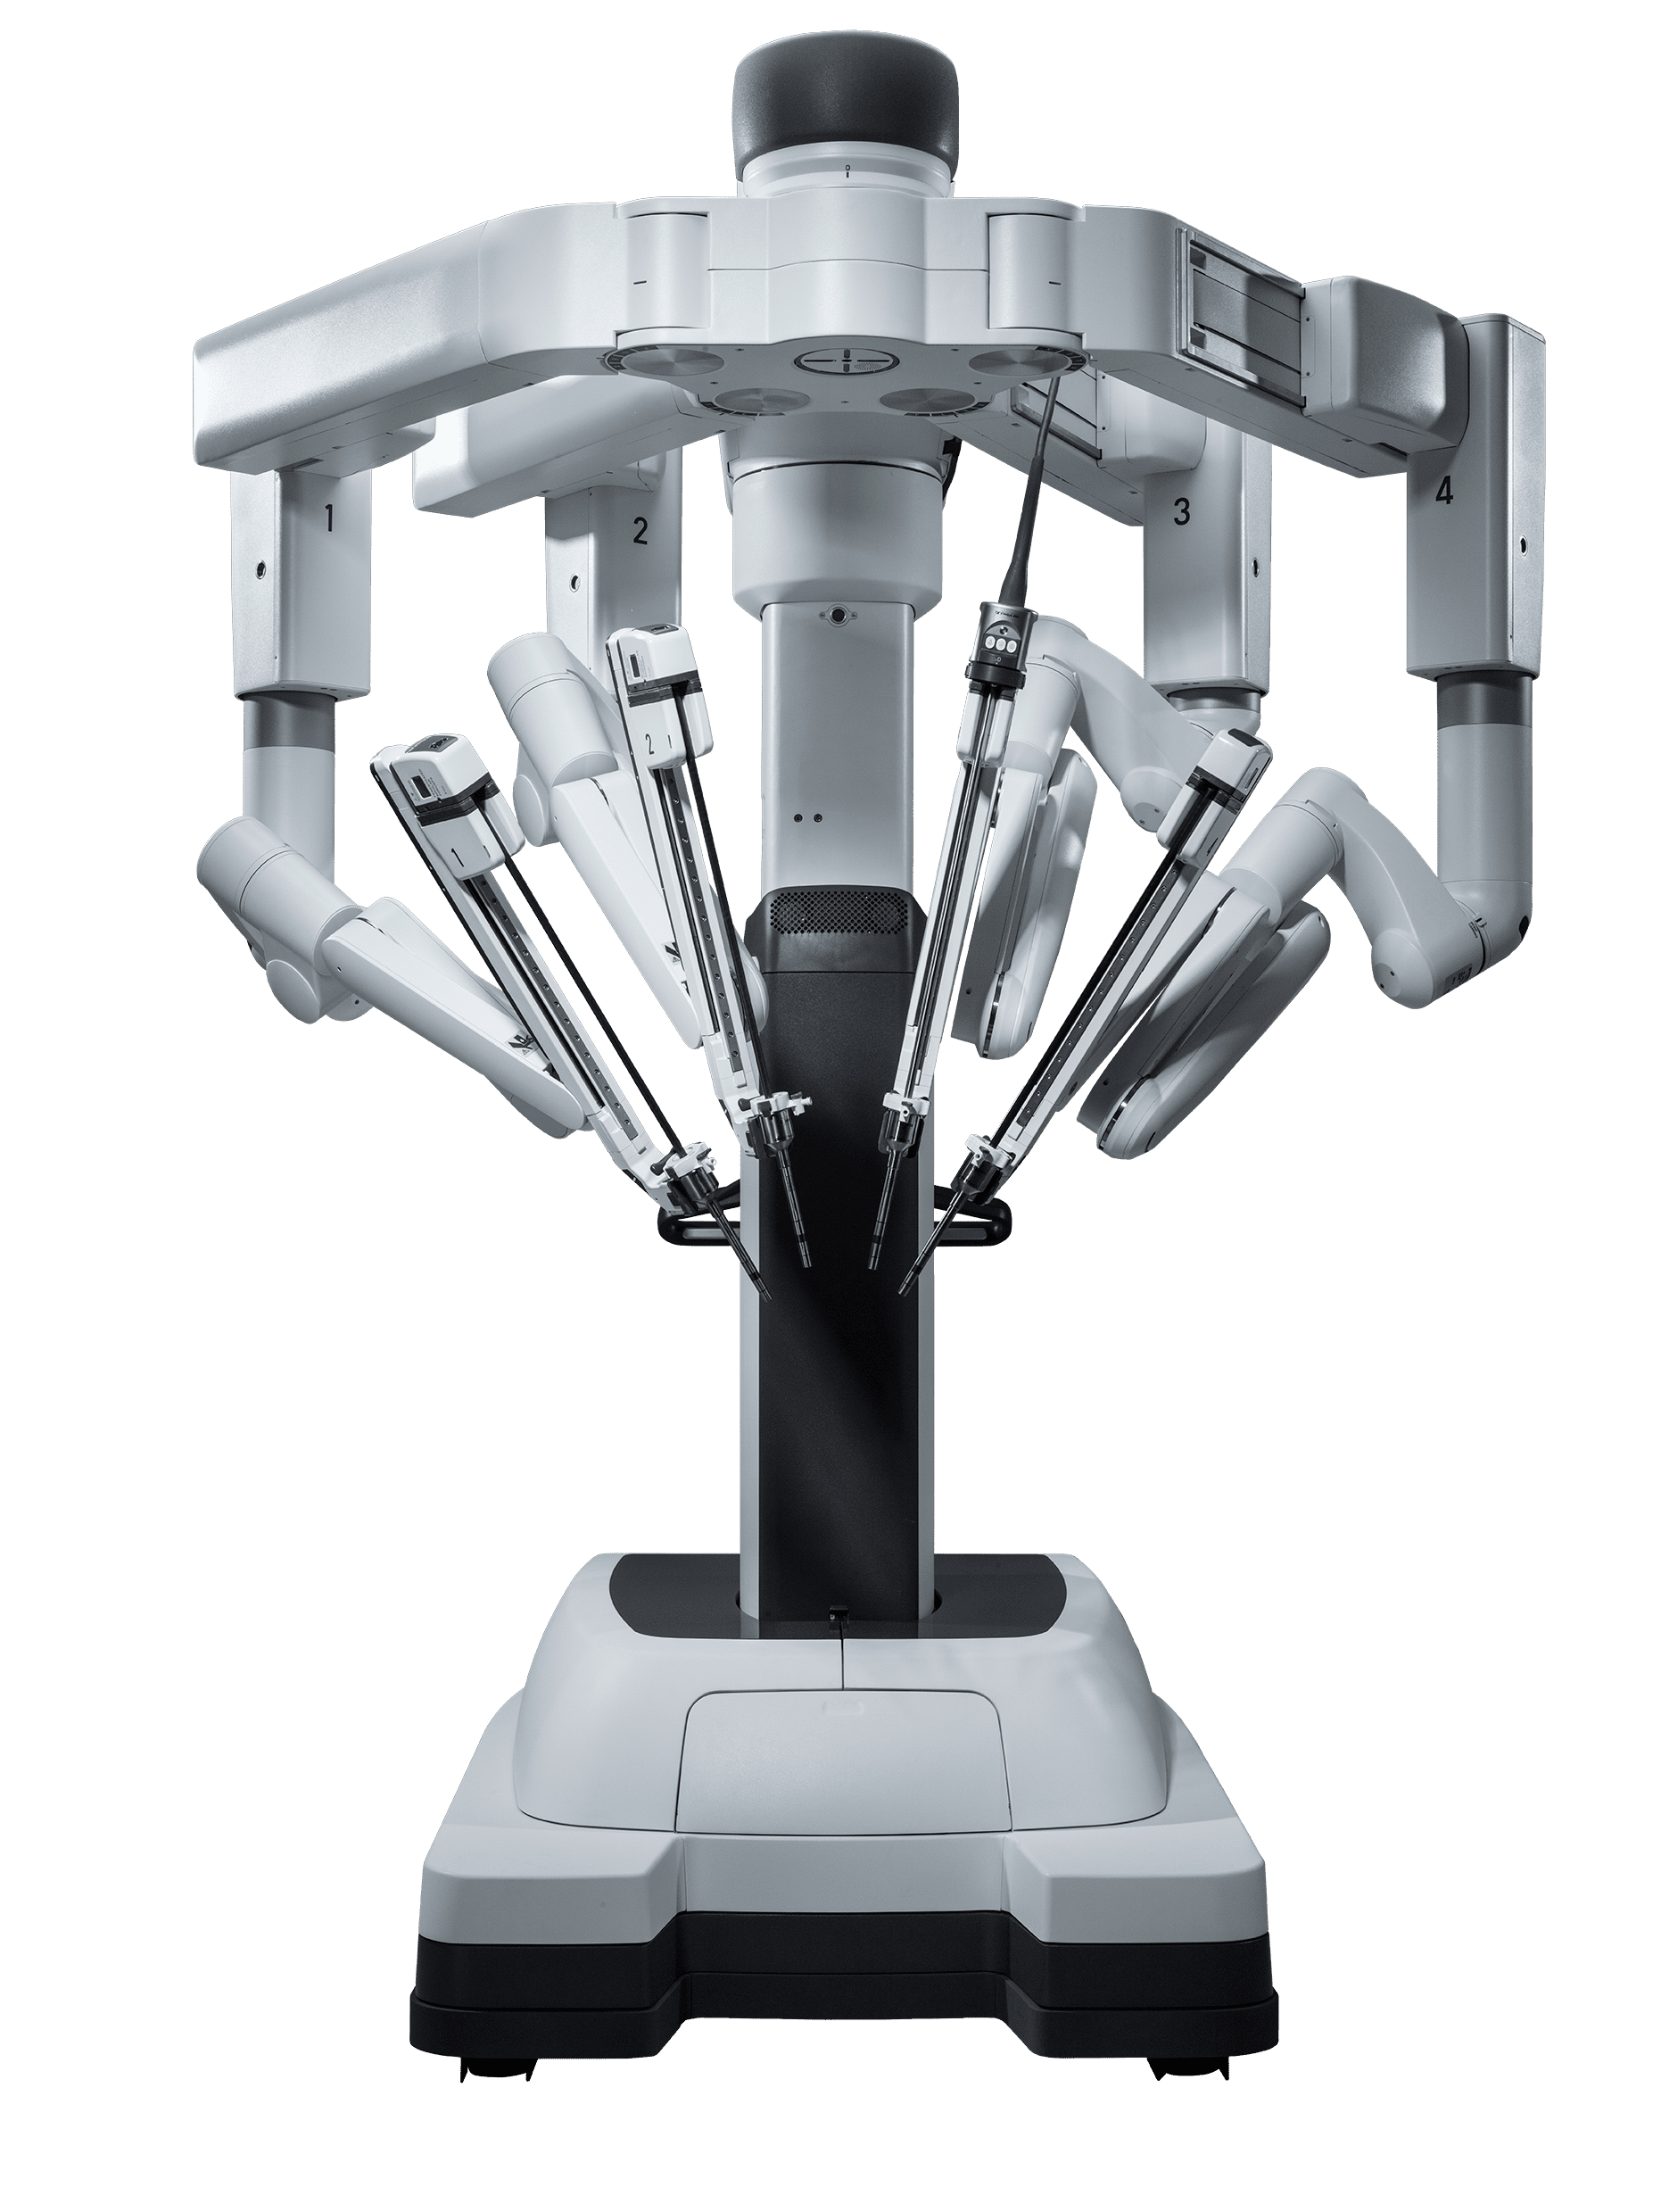
\includegraphics[width=9cm]{images/davinci-xi-patient-cart.png}\\
\caption{DaVinci Xi Patient Cart}
\end{figure}
\end{center}

Surgical robotics have a huge impact in Medicine and Healthcare in general. Some of the advantages are the following:
\begin{itemize}
\item \textbf{Minimally Invasive Procedures} which means
	\begin{itemize}
	\item Smaller incisions
	\item Less blood loss
	\item Reduced risk of inpatient infection
	\item Less pain
	\item Faster patient recovery
	\end{itemize}
\item Increased \textbf{precision} and reduced human errors
	\begin{itemize}
	\item Smooth and precise movements
	\item Detection and correction of errors caused by hand tremble
	\end{itemize}
\item \textbf{No fulcrum effect} and intuitive manipulation of surgical tools
\item \textbf{Haptic feedback}
\item \textbf{Teleoperation} (currently in the same room only): the surgeon operates while they sit on a special \textbf{ergonomic} console, which makes 
the long procedures more comfortable and efficient.
\end{itemize} 

\begin{center}
\begin{figure}[H]
\centering
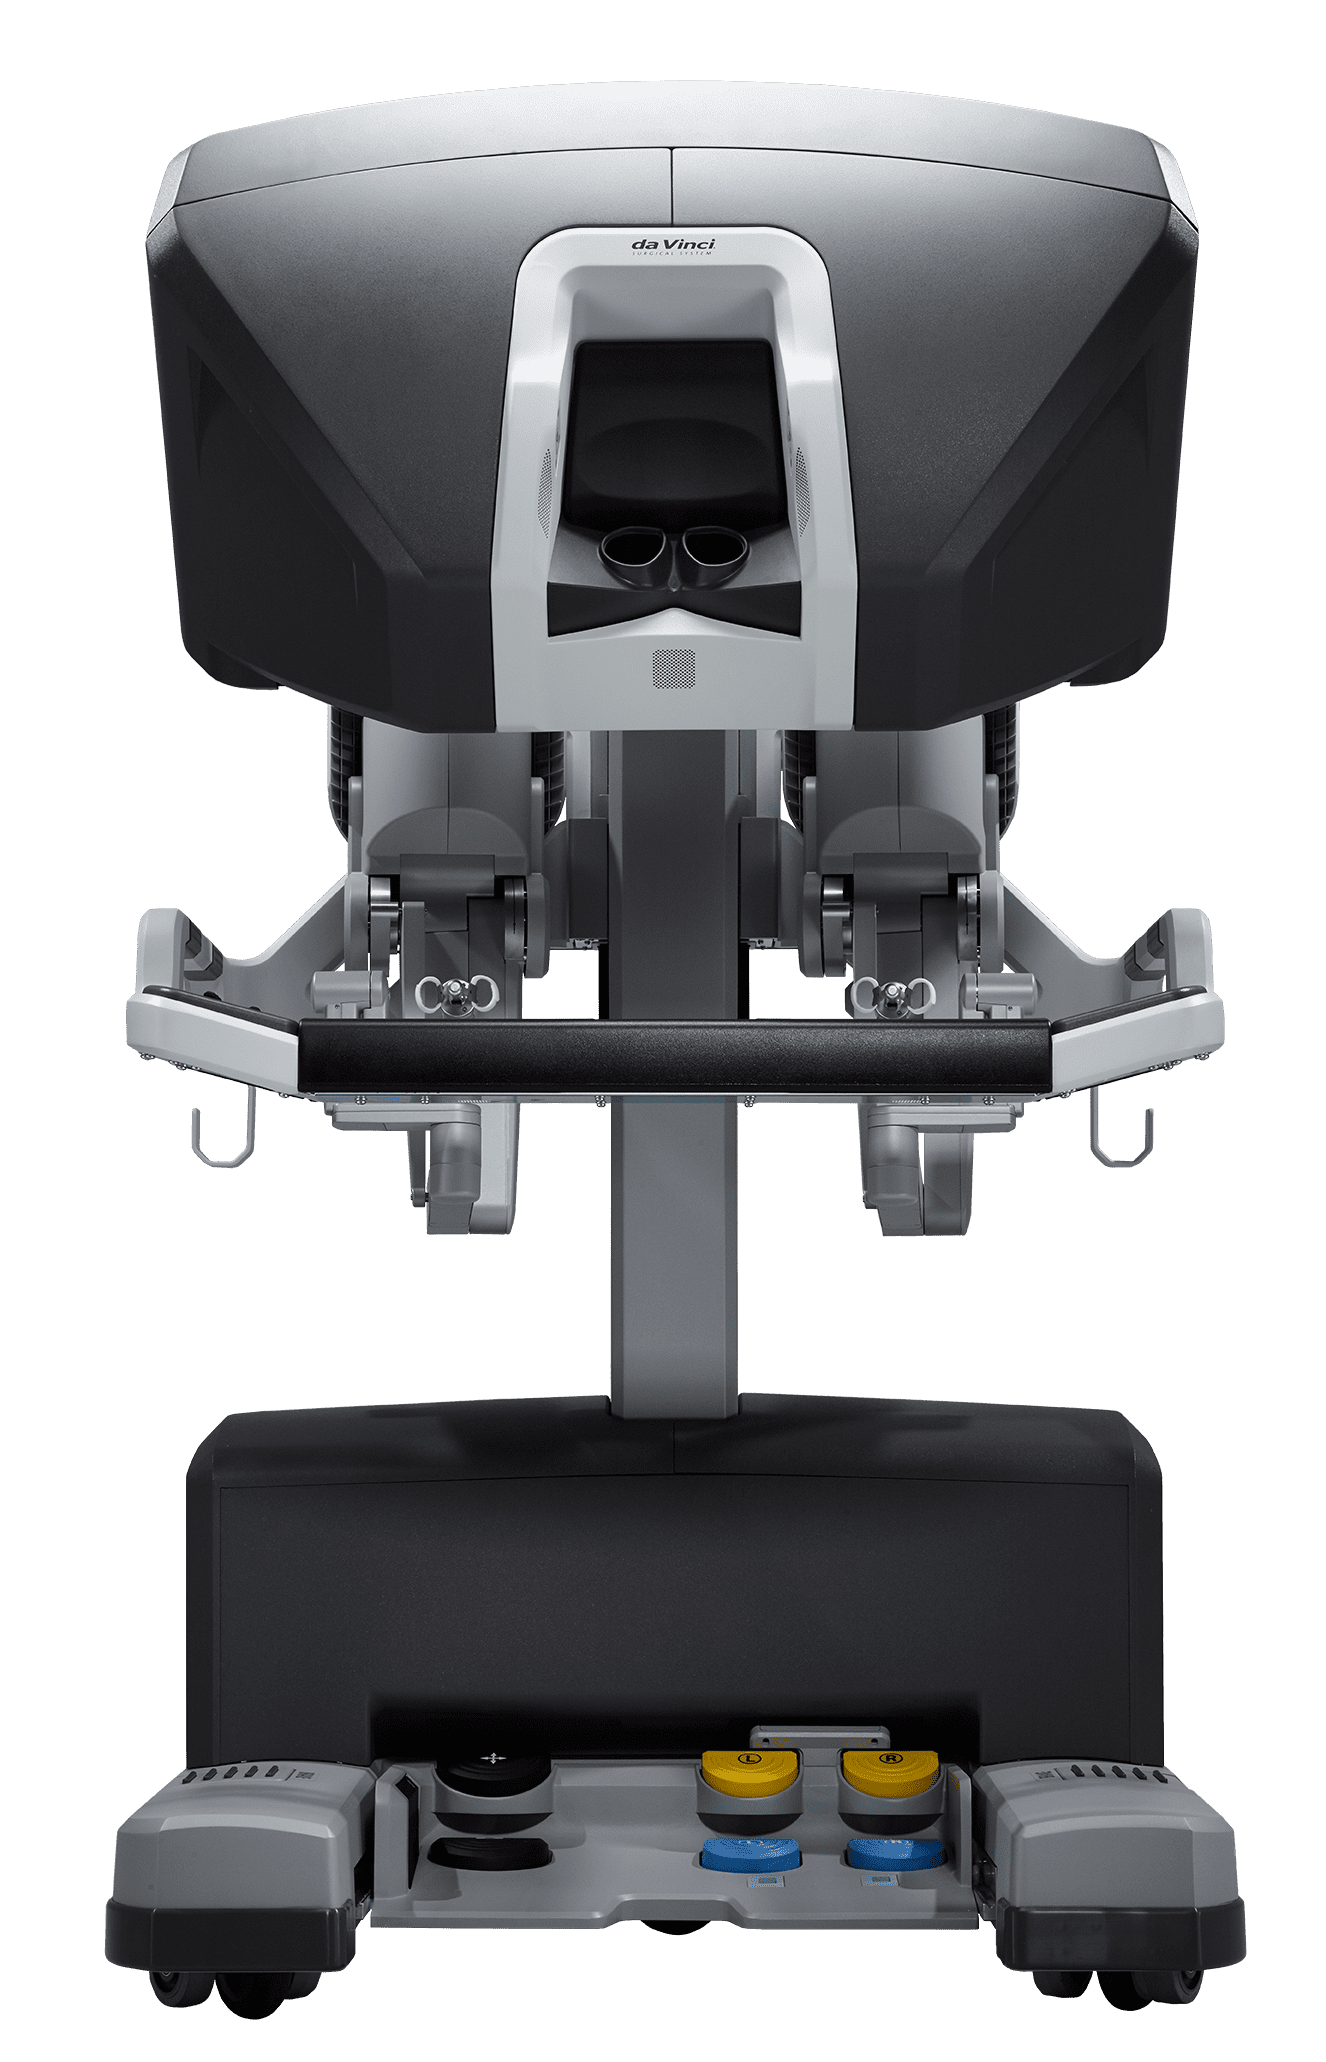
\includegraphics[width=7cm]{images/davinci-xi-surgeon-console.png}\\
\caption{DaVinci Xi Surgeon Console}
\end{figure}
\end{center}

\subsection{Bibliography Overview}

\subsection{Methodology \& Approach}

%\newpage
\section{Robotic arm Kinematic Analysis}


\subsection{Robotic arm, DH parameters \& Forward Kinematics}

\begin{center}
\begin{figure}[H]
\centering
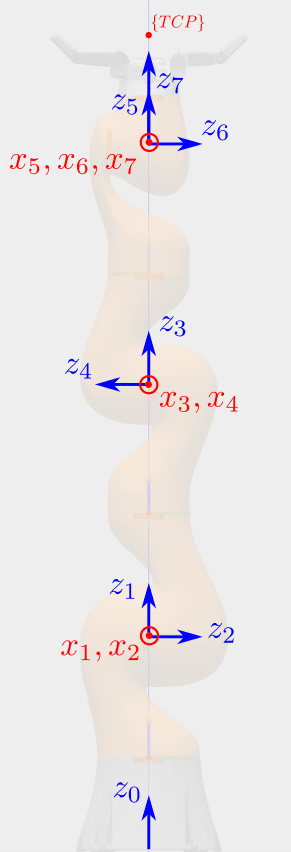
\includegraphics[height=12cm]{images/iiwa-frames.png}\\
\caption{Joint reference frames of the KUKA iiwa14 robot}
\end{figure}
\end{center}

\begin{center}
\begin{tabular}{ |c|c|c|c|c| } 
\hline
i & $θ_i$ (rad) & $L_{i-1}$ (m) & $d_i$ (m) & $α_{i-1}$ (rad) \\
\hline
1 & $θ_1$ & 0 & 0.36 & 0 \\
2 & $θ_2$ & 0 & 0 & $-π/2$ \\
3 & $θ_3$ & 0 & 0.36 & $π/2$ \\
4 & $θ_4$ & 0 & 0 & $π/2$\\
5 & $θ_5$ & 0 & 0.4 & $-π/2$ \\
6 & $θ_6$ & 0 & 0 & $-π/2$ \\
7 & $θ_7$ & 0 & 0 & $π/2$ \\
\hline
\end{tabular}
\end{center}

\[
^{i-1}T_i = 
\begin{bmatrix}
c\theta_i & -s\theta_i & 0 & L_{i-1} \\
s\theta_ica_{i-1} & c\theta_ica_{i-1} & -sa_{i-1} & -sa_{i-1}d_i \\
s\theta_isa_{i-1} & c\theta_isa_{i-1} & ca_{i-1} & ca_{i-1}d_i \\
0 & 0 & 0 & 1\\
\end{bmatrix}
\]


\subsection{Inverse Kinematics}

\subsubsection{Decoupling Technique}

In this section the inverse kinematics problem is solved for only the 6 out of the 7 total degrees of freedom. The third joint is not used in this 
analysis and it's angle is set to zero $θ_3 = 0$ . The rest of the joints form a special kind of kinematic chain that can be solved using the 
decoupling technique. In this technique the Inverse kinematics problem is split to 2 separate subproblems, one for the position and one for the 
orientation of the end-effector. This technique can be applied in this case because the axes of the 3 last joints intersect at the same point and 
they form an Euler wrist. \\

To solve for the joints' angles, the transformation matrix $^0T_7$ of the end-effector with respect to the robot's base is required. Usually the transformation ${}^UT_{tcp}$ is known, which is the pose of Tool's center point (TCP) with respect to the Universal Coordinate Frame $\lbrace U \rbrace$ from which the required $^0T_7$ can be calculated

\[
{}^UT_{tcp} = {}^UT_0  \;\;  {}^0T_7  \;\;   {}^7T_{tcp}
\]
\[
{}^0T_7 = {}^UT_0^{-1}  \;\;  {}^UT_{tcp}  \;\;  {}^7T_{tcp}^{-1}
\]
\[
{}^0T_7 = \begin{bmatrix}
R_t & \mathbf{p}_t \\
0 & 1 \\
\end{bmatrix}
\]

where ${}^UT_0,  \;\;   {}^7T_{tcp}$ are translation transformations by a constant distance and $R_t,  \;\; \mathbf{p}_t$ are the target's orientation 
and position respectively.

\[
{}^0\mathbf{p}_5 = {}^0T_4 {}^4\mathbf{p}_5 = \begin{bmatrix} p_x \\ p_y \\ p_z \\ \end{bmatrix}
\]

\begin{equation}
θ_1 = 
\begin{cases}
atan2 \left( p_y, p_x \right) \\
π - atan2 \left( p_y, p_x \right)
\end{cases}
\end{equation}

\begin{center}
\begin{figure}[H]
\centering
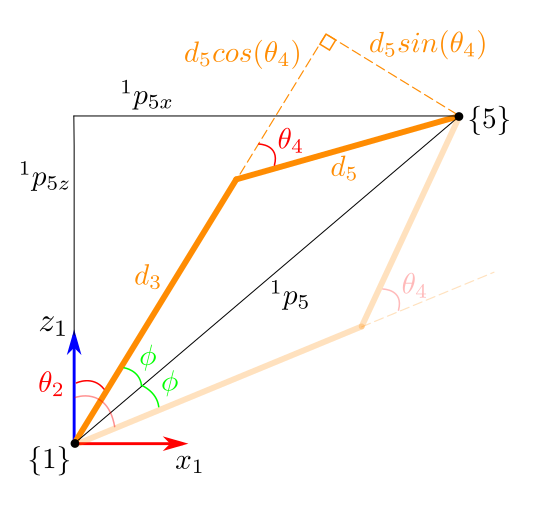
\includegraphics[width=8cm]{images/th2-4-calculation.png}\\
\caption{Calculation of angles $θ_2, θ_4$}
\end{figure}
\end{center}

\[
φ = acos \left( \frac{d_3^2 + \Vert{}^1p_{5}\Vert ^2 - d_5^2}{2d_3 \Vert{}^1p_{5}\Vert} \right)
\]
\begin{equation}
θ_2 = atan2 \left( \sqrt{p_x^2 + p_y^2}, {}^1p_{5z} \right) \pm φ
\end{equation}

\[ c_4 = \frac{ \Vert{}^1p_{5}\Vert ^2 - d_3^2 - d_5^2 }{2d_3d_5} \]
\begin{equation}
θ_4 = atan2 \left( \pm \sqrt{1 - c_4^2}, c_4 \right)
\end{equation}

Once $θ_1,θ_2,θ_3,θ_4$ are known, the orientation matrix of the wrist can be calculated as following
\[
R_{target} = 
\begin{bmatrix}
i_x & j_x & k_x\\
i_y & j_y & k_y\\
i_z & j_z & k_z\\
\end{bmatrix}
\]
\begin{equation}
θ_6 = atan2 \left( \pm \sqrt{1-k_y^2}, k_y \right)
\end{equation}
\[
θ_7 = atan2 \left( -j_y, i_y \right)
\]
\[
θ_5 = atan2 \left( - k_z, k_x \right)
\]


\subsubsection{Workspace constraints \& Singularity points}

\begin{center}
\begin{figure}[H]
\centering
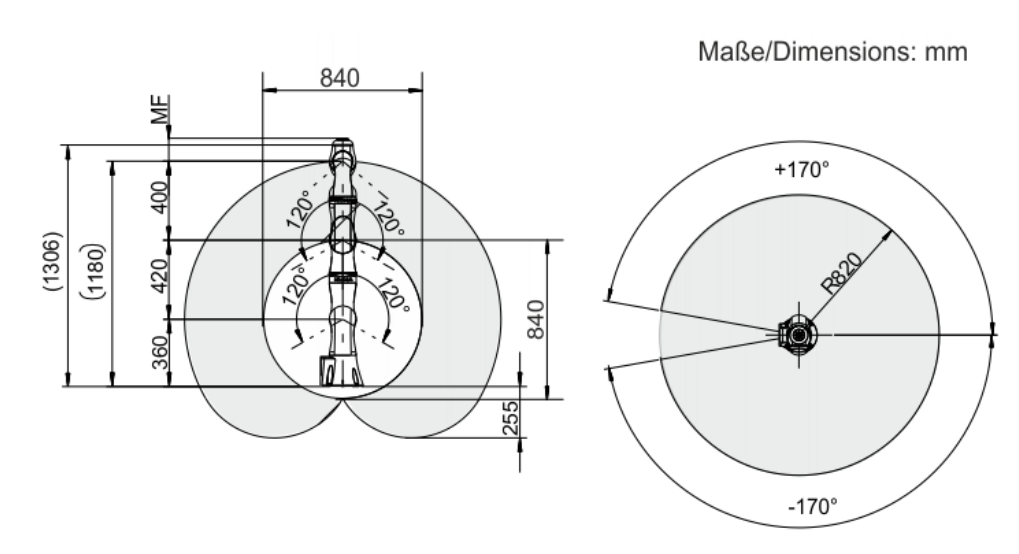
\includegraphics[width=10cm]{images/iiwa-workspace.png}\\
\caption{KUKA iiwa LBR14 workspace dimensions}
\end{figure}
\end{center}

Singularity points:
\begin{itemize}
	\item When $p_x^2 + p_y^2 = 0$ then the end-effector lies on the z-axis and $θ_1$ is not defined
	\item When $sin\left( θ_6 \right) = 0$ then the angles $θ_5, θ_7$ are not defined
\end{itemize}

\subsubsection{Solutions for 7DoF numerically}

\subsubsection{Comparison of Inverse Kinematics Techniques}


%\newpage
\section{Grasping}

\subsection{Gripper \& Forward Kinematics}

\begin{center}
\begin{figure}[H]
\centering
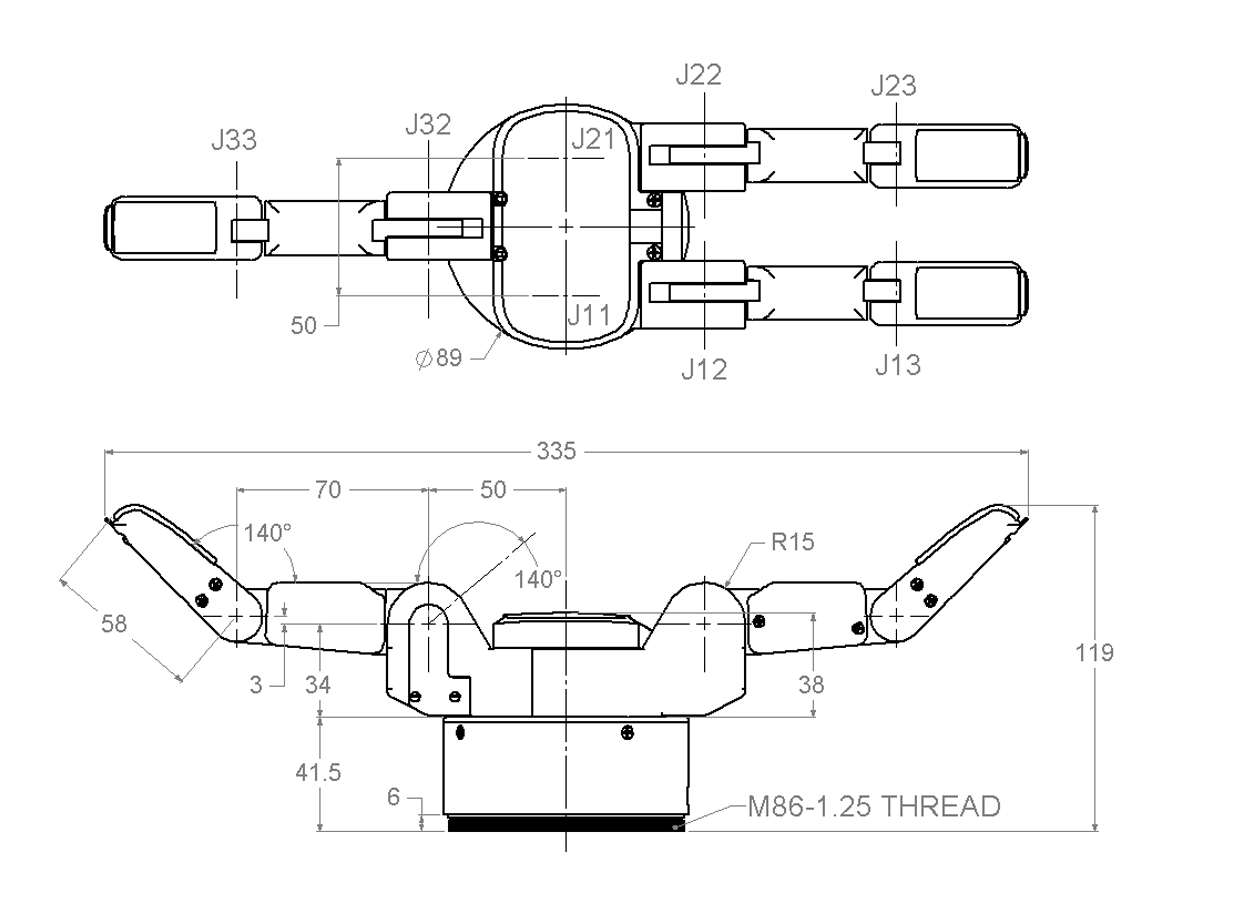
\includegraphics[width=12cm]{images/bh8-282-dimensions.png}\\
\caption{Barrett Hand gripper (model BH8-282) dimensions}
\end{figure}
\end{center}


\subsection{Gripper Inverse Kinematics}

The following Inverse Kinematics analysis referes to one finger of the Barrett Hand gripper, which has 3 revolute joints. Finger 3 has only 2 
revolute joints for which the angle solutions are the same with the solutions of the last 2 joints of the other fingers. Let

\[
\mathbf{p} = \begin{bmatrix} p_x \\ p_y \\ p_z \\ \end{bmatrix}
\]

be the position of the grasp point for one finger. The first angle can easily be calculated as

\begin{equation}
φ_1 = atan2 \left( p_y, p_x \right)
\end{equation}

Next, we calculate the third angle based on the law of cosines (see fig.)
\[
cos \left( π - φ_3 - \frac{π}{4} \right) = \frac{L_2^2 + L_3^2 - p^2}{2 L_2 L_3}
\]
\[
cos \left(φ_3 + \frac{π}{4} \right) = \frac{p^2 - L_2^2 - L_3^2}{2 L_2 L_3}
\]
\begin{equation}
φ_3 = atan2 \left[ \pm \sqrt{1 - \left( \frac{p^2 - L_2^2 - L_3^2}{2 L_2 L_3} \right)^2} , \frac{p^2 - L_2^2 - L_3^2}{2 L_2 L_3} \right] - \frac{π}{4}
\end{equation}

In a more general case, the first argument of the $atan2$ function in the expression of $φ_3$ could also be negative,
but in this case this second solution is rejected, because due to mechanical constraints, this angle can't be negative. 
After having calculated $φ_3$ we can calculate $φ_2 $

\[
tan \left( ψ + φ_2 \right) = \frac{p_z}{\sqrt{p_x^2 + p_y^2}}
\]
\[
tan \left( ψ \right) = \frac{L_3 sin \left( φ_3 + \frac{π}{4} \right) }{L_2 + L_3 cos \left( φ_3 + \frac{π}{4} \right)}
\]

\begin{equation}
φ_2 = atan2 \left( pz, \sqrt{p_x^2 + p_y^2} \right) - atan2 \left[ L_3 sin \left( φ_3 + \frac{π}{4} \right), L_2 + L_3 cos \left( φ_3 + \frac{π}{4} \right) \right]
\end{equation}

\subsection{Force closure}
The planar case, the spatial case \& convex hull test.

\lstinputlisting[frame=single,basicstyle=\ttfamily\small\color{blue},caption=Example ROS message with collision/contact information between one finger of the gripper and one surgical tool]{data/collision-contact-ros-message-example1.txt}

%\newpage
\section{Scene and object recognition with Computer Vision and Visual Servoing}

At this section we explore ways to detect and recognize the surgical tools as well as other objects of the simulation scene. To reduce the complexity of 
this thesis and focus on the more important features of this thesis, we assume in the simulation that the surgical tools are blue and the mounting dock, 
where the tools will be placed, is green. These assumptions make the scene and object recognition much easier without the need of more advanced image 
processing and/or machine learning recognition algorithms.\\

\textbf{Camera setup} used in this thesis:
\begin{itemize}
\item 2 HD RGB cameras with resolution $1280 \times 720$
\item near clipping plane: 0.02
\item far clipping plane: 300 
\item horizontal FoV (field of view): 1.396
\item update rate: 30fps
\end{itemize}

\subsection{Laparoscopic tool detection}

In order to detect the shape of the tool there are some standard steps that need to be executed. After having loaded the input image we convert it to grayscale, so that we can work on only one channel instead of
3 color channels and thus reduce the amount of calculations. Also for the purposes of extracting the shape of an object, the color doesn't have a very significant role in the algorithm. Next step is 
to remove the unwanted noise. In this thesis we only assume that the video frames have only Additive White Gaussian Noise (AWGN). To remove some of the
noise we use a moving average filter (the filter is also known as a kernel), which is convoluted around the whole image. The filter that was used is the following 3-by-3 matrix
\[
h = \frac{1}{9} \begin{bmatrix}
1 & 1 & 1 \\
1 & 1 & 1 \\
1 & 1 & 1 \\
\end{bmatrix}
\]
the output, filtered image is the result of the convolution of the image with the filter and is calculated as following
\[
g(i,j) = \sum_{k,l} f(i+k,j+l)h(k,l)
\]
where $g(\cdot, \cdot)$ is the output image and $f(\cdot, \cdot)$ is the input image.

After the noise is removed the image is getting binarized. To do that, we set a threshold, below which the pixels will be black and the rest will be white. This conversion to binary format, makes it 
easier to extract the boundaries of the black shapes, which will correspnd to the boundaries of the objects of the initial image.

\begin{center}
\begin{figure}[H]
\centering
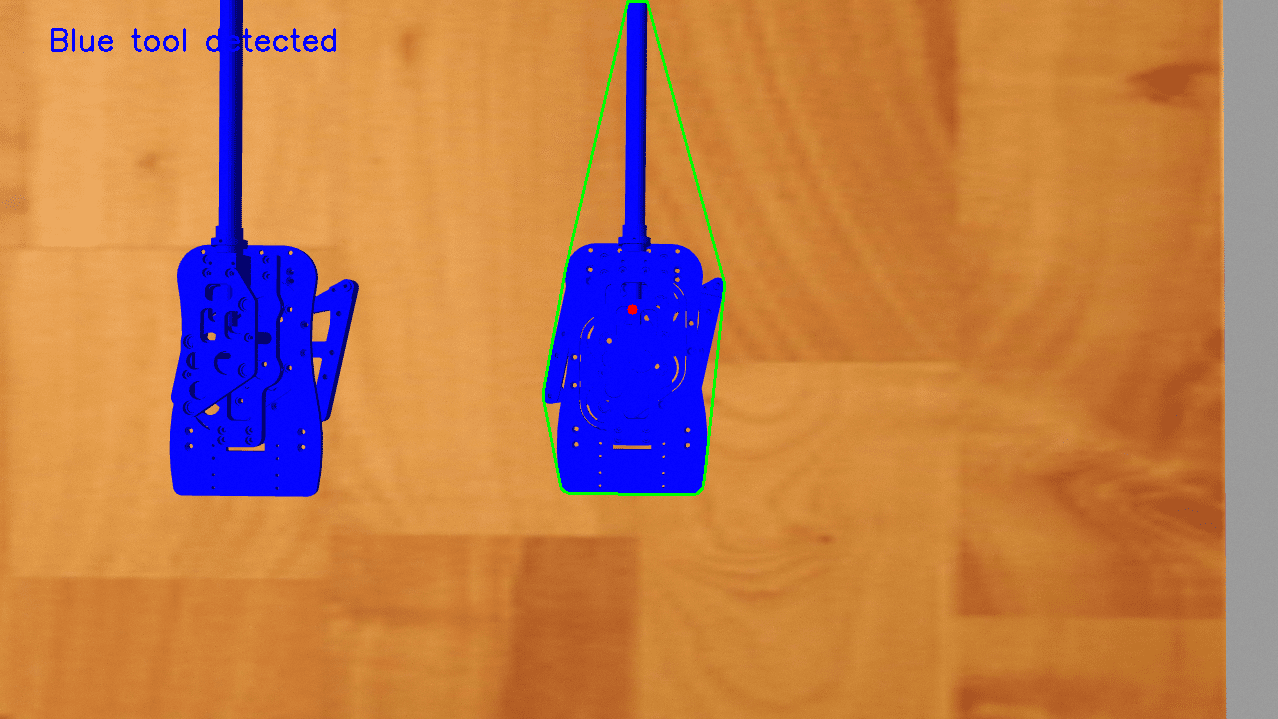
\includegraphics[width=12cm]{images/opencv-tool-convex-hull.png}\\
\caption{Simple tool detection in simulation based on color, using OpenCV. The green polygon is the convex hull, and the red point is the
estimated center of mass}
\end{figure}
\end{center}

\subsection{Stereoscopic vision}

\begin{center}
\begin{figure}[H]
\centering
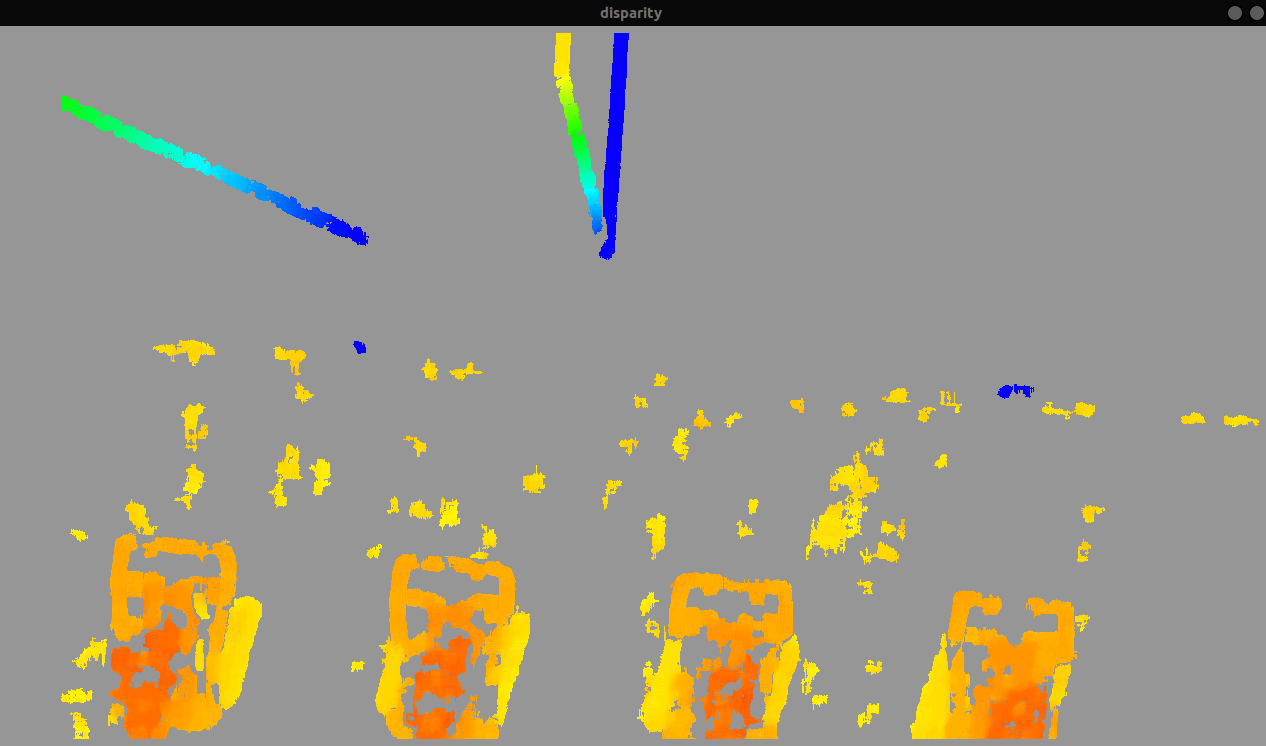
\includegraphics[width=12cm]{images/disparity.png}\\
\caption{Disparity image calculated from the 2 cameras}
\end{figure}
\end{center}

\begin{center}
\begin{figure}[H]
\centering
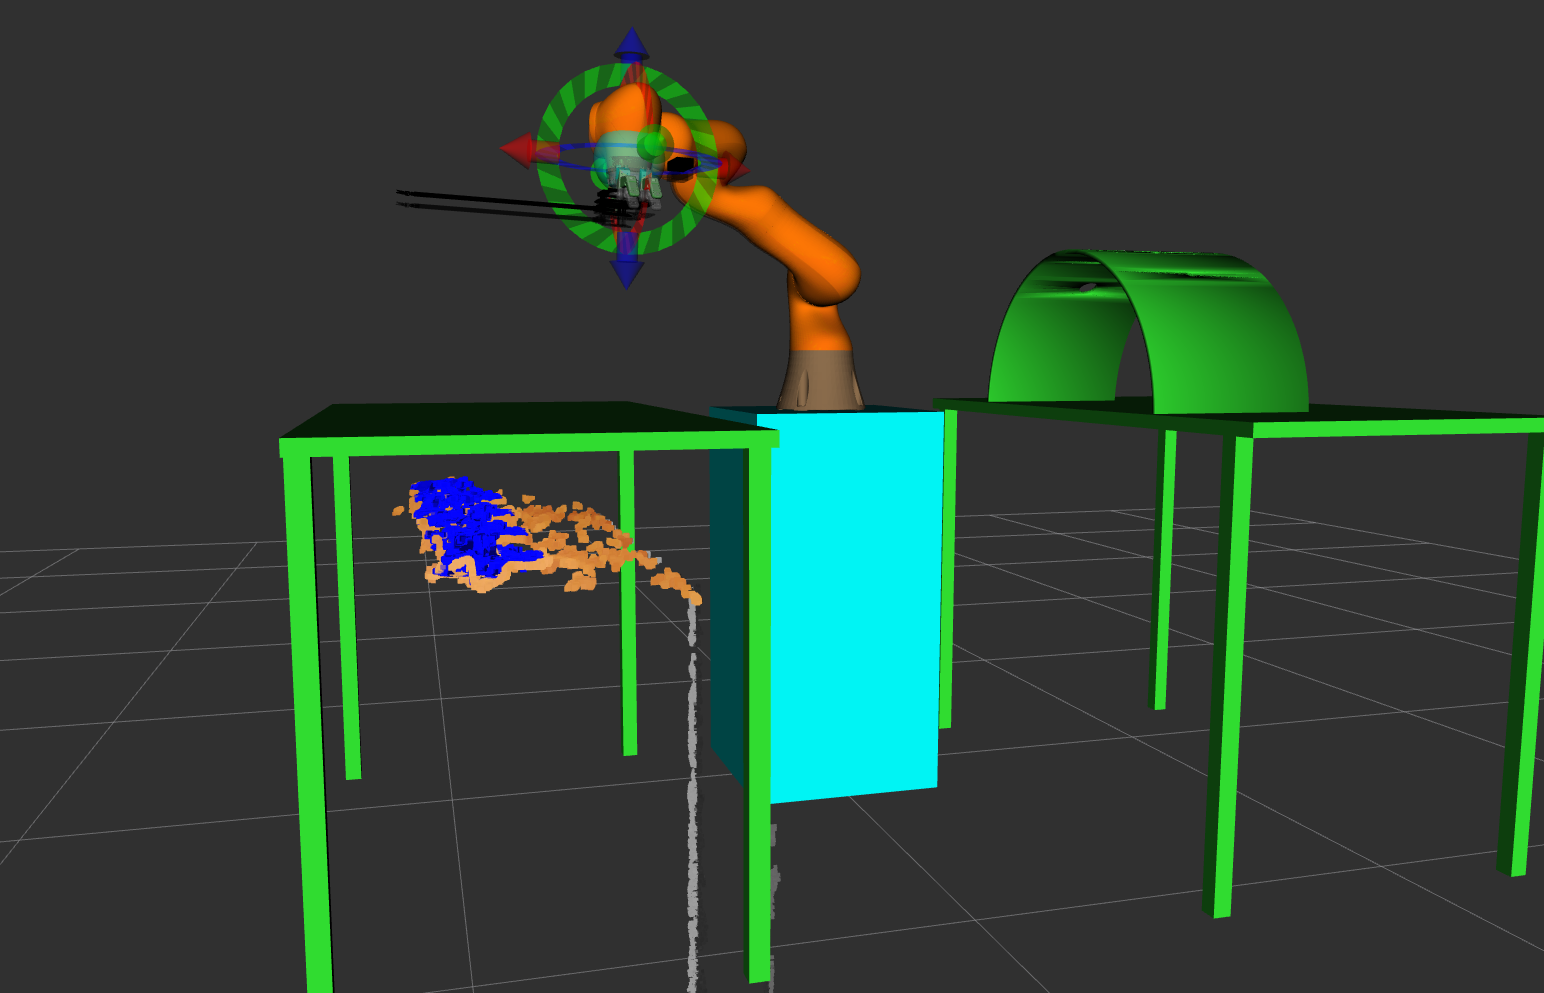
\includegraphics[width=12cm]{images/point_cloud.png}\\
\caption{Point cloud of surgical tools, generated from the 2 cameras and visualized in RViz}
\end{figure}
\end{center}

\subsection{Calculation of tool position and orientation}

In order for the gripper to grasp correctly the laparoscopic tool, it is required to calculate the tool's position and orientation in the pixel space 
which must then be converted with respect to the robot's workspace. From all the pixels that have been classified as part of the laparoscopic tool, 
one can estimate the center of mass and two perpendicular vectors 
attached to that point that define the orientation. The center of mass is simply the average of the $(x,y)$ coordinates of all the tool's pixels
\[
\left( \bar{x}, \bar{y} \right) = \left( \frac{1}{N}\sum_{i=1}^{N} x_i , \frac{1}{N}\sum_{i=1}^{N} y_i \right)
\]

The easiest way to calculate the center of mass is by calculating the average using the first moments of the contour points. However, since the contour is only using
the boundary of the object and not it's area, this method is not very accurate. To get a more accurate value for the center of mass, one must use the pixels that are inside 
the detected object's contour. The simplest way (but most expensive) to get the inside pixels of the tool is to loop over all the pixels and for each pixel check if it is inside the 
polygon (point inside polygon test). To make this method even faster, one can take a sample of the total pixels, for example check one in every 10 pixels in the x and y coordinates, 
which means reducing the time complexity to one tenth. \\

Taking this approach a step further in optimization, one can iterate not in all the video frame pixels but only those pixels 
that are inside the \textbf{Region of Interest} of the tool. The Region of Interest, also known as ROI, is a widely used structure in computer vision and is simply a bounding box (rectangle) that fits exactly 
(or is a bit bigger than) an object or part of the image frame that we want to study. Having already calculated the contour of the surgical tool and it's convex hull we can easily calculate this bounding box. 
For this calculation we prefer to use the convex hull, because it often contains much less pixels than the contour. We iterate over all the pixels of the convex hull and we get the minimum and maximum x and y 
coordinates. The combination of these four values is the desired ROI. Since we now have access to the tool's ROI, we can iterate and sample the pixels inside it (and not all pixels as we did before) to get 
some of the pixels of the tool so that we can more accurately calculate it's center of mass and orientation vectors. \\

The two orientation vectors are the eigenvectors of the covariance matrix of the above pixels. Let $\mathbf{a},\mathbf{b}$ be the orientation vectors, 
then $\mathbf{a},\mathbf{b}$ are solutions of the equation
\[
C \mathbf{v} = λ \mathbf{v}
\]
where $C$ is the covariance matrix given by
\[
C = \begin{bmatrix}
σ(x,x) & σ(x,y) \\
σ(y,x) & σ(y,y) \\
\end{bmatrix}
\]
\[
σ(x,y) = \frac{1}{n-1} \sum_{i=1}^{N} ( x_i - \bar{x} )( y_i - \bar{y} )
\]

\begin{center}
\begin{figure}[H]
\centering
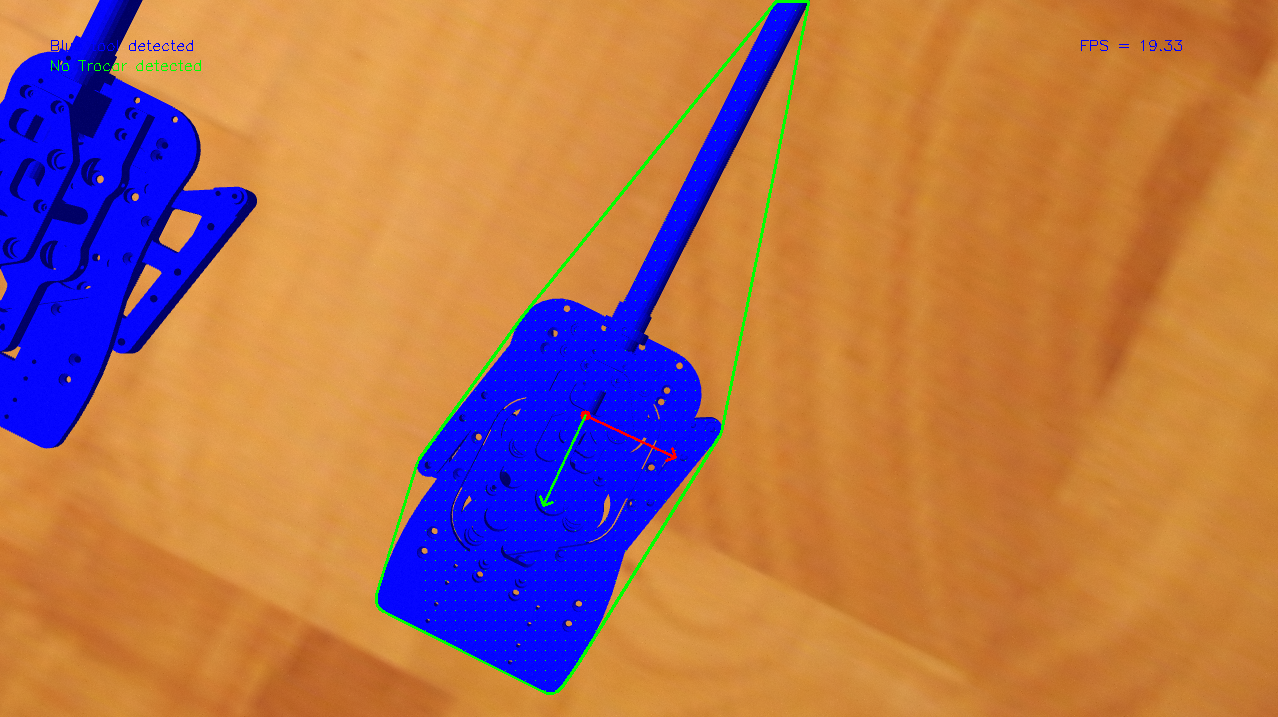
\includegraphics[width=0.8\textwidth]{images/tool-pose.png}\\
\caption{Estimation of tool's pose (position and orientation). The red dot is the center of mass and attached to that are the two orientation vectors of the tool. The green polygon is the convex hull of the tool 
and the white rectangle is it's ROI as calculated from the convex hull}
\end{figure}
\end{center}

\subsection{Calculation of grasping points}

\subsection{Trocar detection \& Estimation of fulcrum point}

\begin{center}
\begin{figure}[H]
\centering
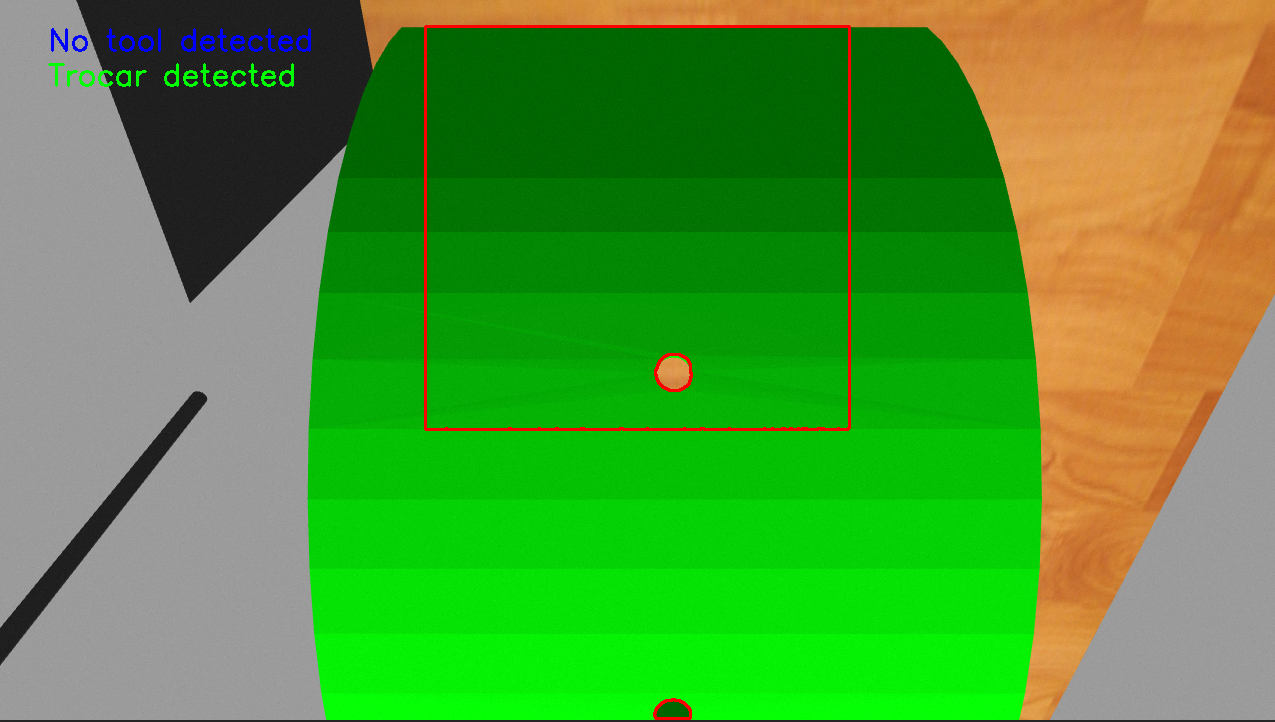
\includegraphics[width=12cm]{images/opencv-trocar-detection.png}\\
\caption{Simple trocar detection in simulation based on color, using OpenCV. In simulation, the trocar is simply considered to be a small 
cylindrical hole and it's center is the fulcrum point}
\end{figure}
\end{center}

\subsection{Visual Servoing}

At this chapter we briefly investigate how visual servoing can be applied in surgery robotics. \textbf{Visual Servoing} is the use of visual information 
to guide and control a robot. The main task of visual servoing is to control the end-effector's pose using features extracted from visual information. The 
features that are usually extracted from cameras are the position and orientation of the detected object, the distance of the object from the camera (using 
stereoscopic vision, photogrammetry or other techniques), the size and the shape of the object. The visual servoing can be executed either in the robot's space 
using position-based servoing or in the camera's space (also known as "pixel space") by using the image-based technique.

\subsubsection{Position based servoing}

\begin{center}
\begin{figure}[H]
\centering
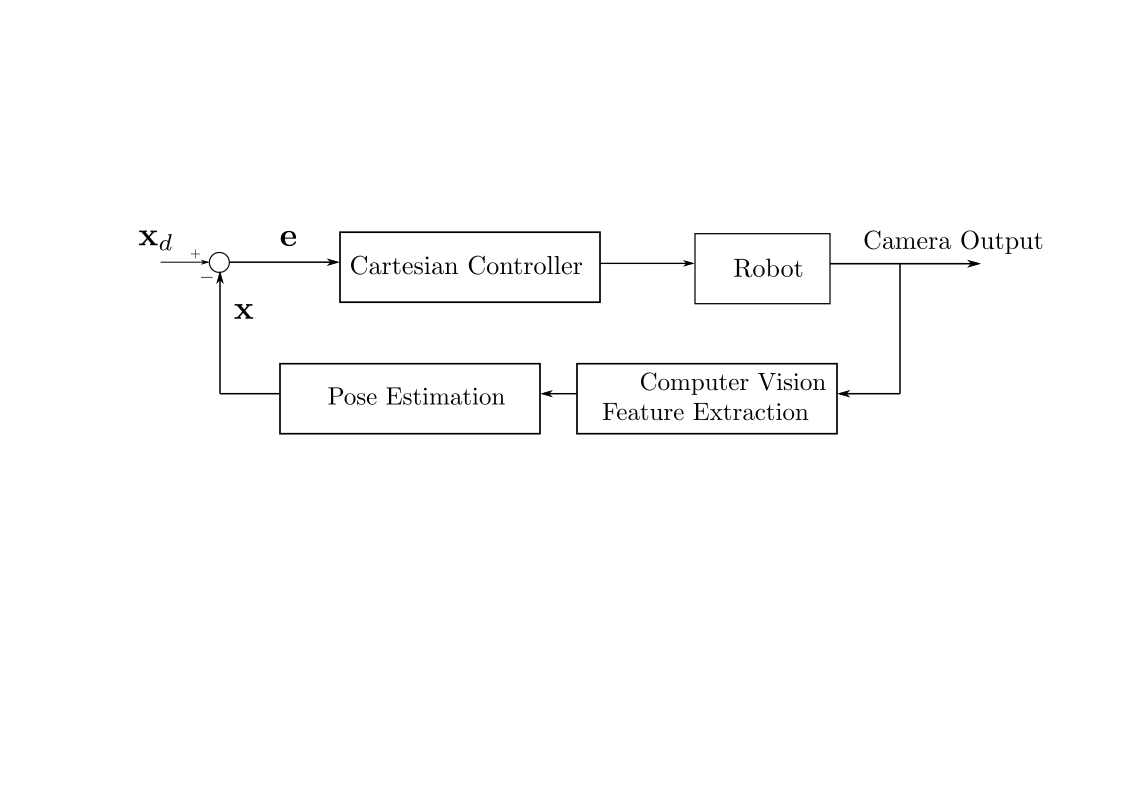
\includegraphics[width=0.8\textwidth]{images/visual-servoing-position-based.png}\\
\caption{Position based visual servoing closed loop control}
\end{figure}
\end{center}

\begin{itemize}
\item \textbf{Photogrammetric technique}
\item \textbf{Stereoscopic vision}
\item \textbf{Extracting depth from motion}
\end{itemize}

\subsubsection{Image based servoing}

\begin{center}
\begin{figure}[H]
\centering

\includegraphics[width=0.8\textwidth]{images/visual-servoing-image-based.png}\\
\caption{Image based visual servoing closed loop control}
\end{figure}
\end{center}

\begin{center}
\begin{figure}[H]
\centering
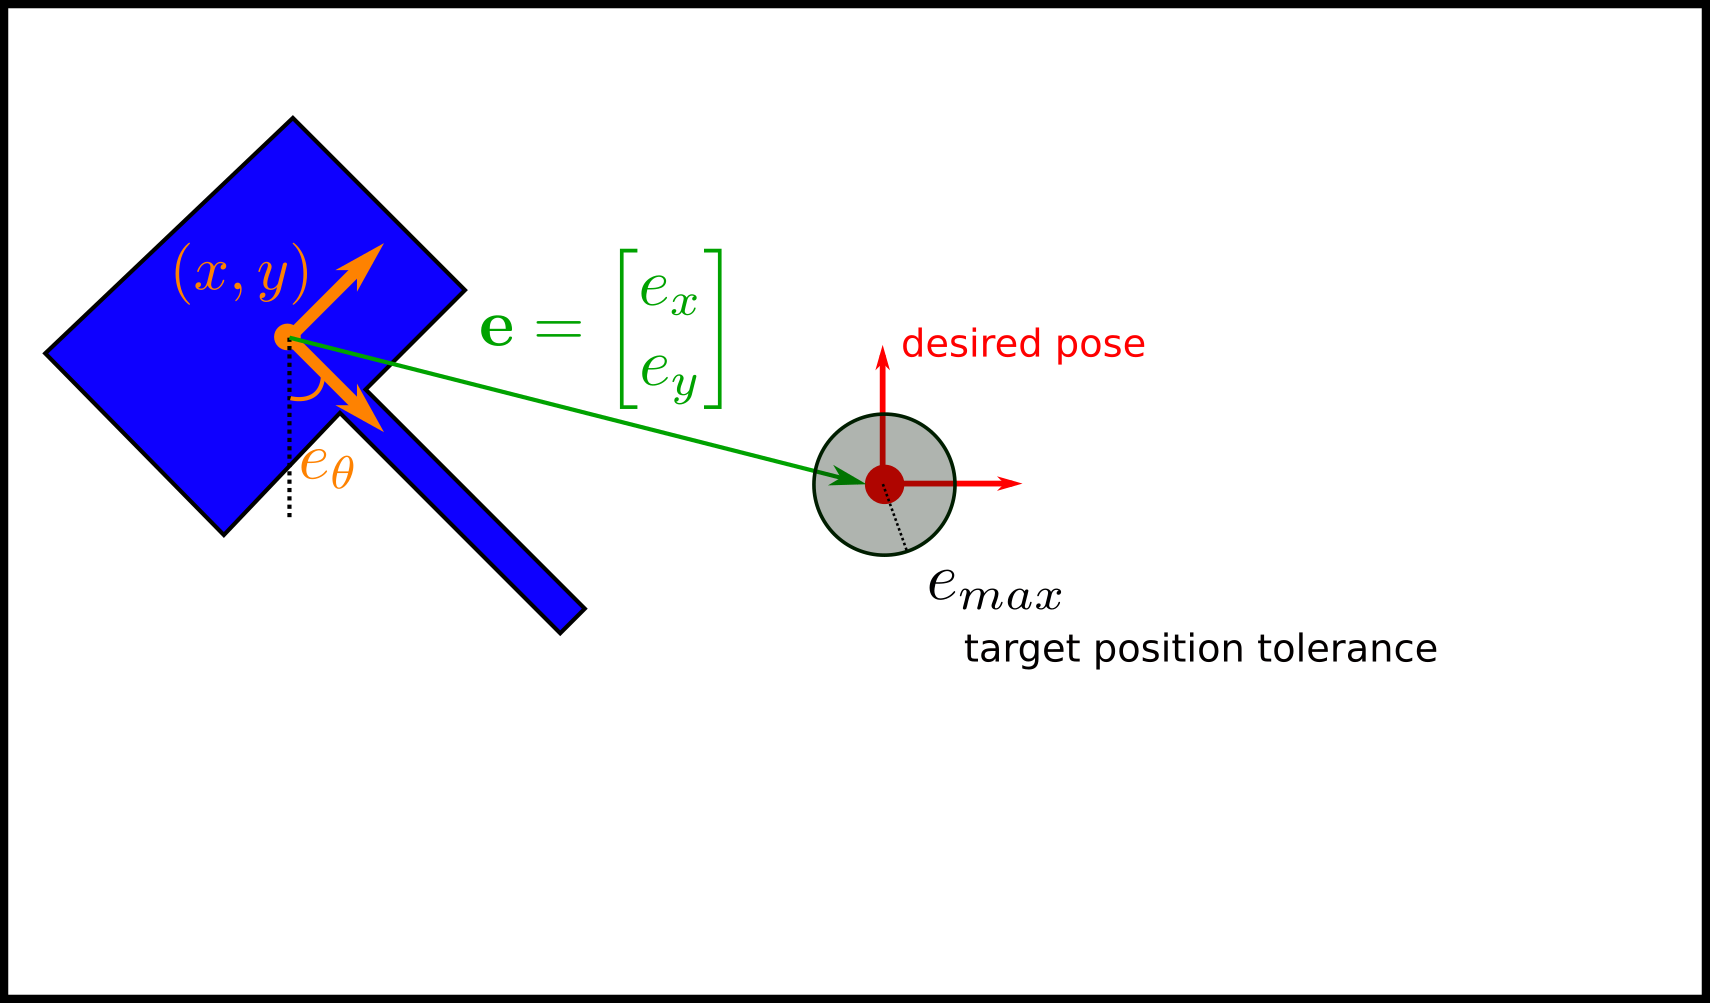
\includegraphics[width=0.45\textwidth]{images/visual_servo_start.png}
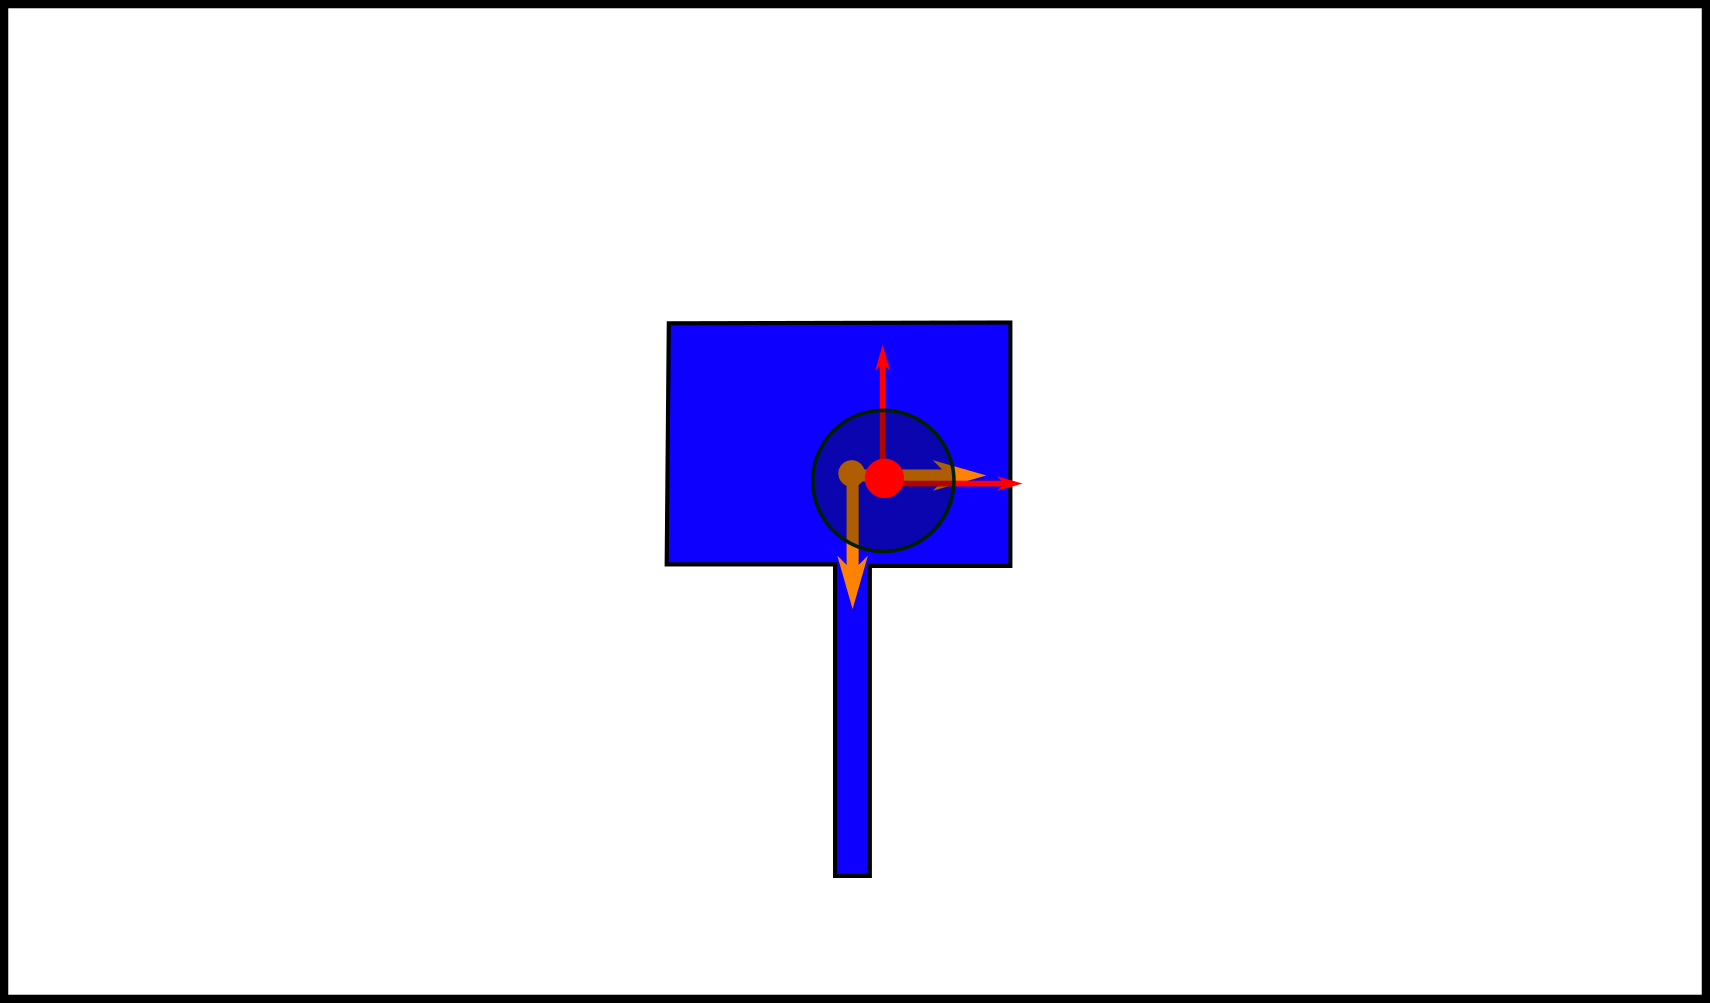
\includegraphics[width=0.45\textwidth]{images/visual_servo_end.png}\\
\caption{Image based visual servoing. The robot arm is controlled using the information gained from the video frames. The frames are 2Dimensional and thus 
the detected objects can have only 3 degrees of freedom which means we can mainly control 3 independent variables, here the $x,y,θ$ variables. The left image 
is the initial frame and the right image is the frame where the object is at the target pose.}
\end{figure}
\end{center}


%\newpage
\section{Laparoscopic tool manipulation}

\subsection{Tool pose}

\begin{center}
\begin{figure}[H]
\centering
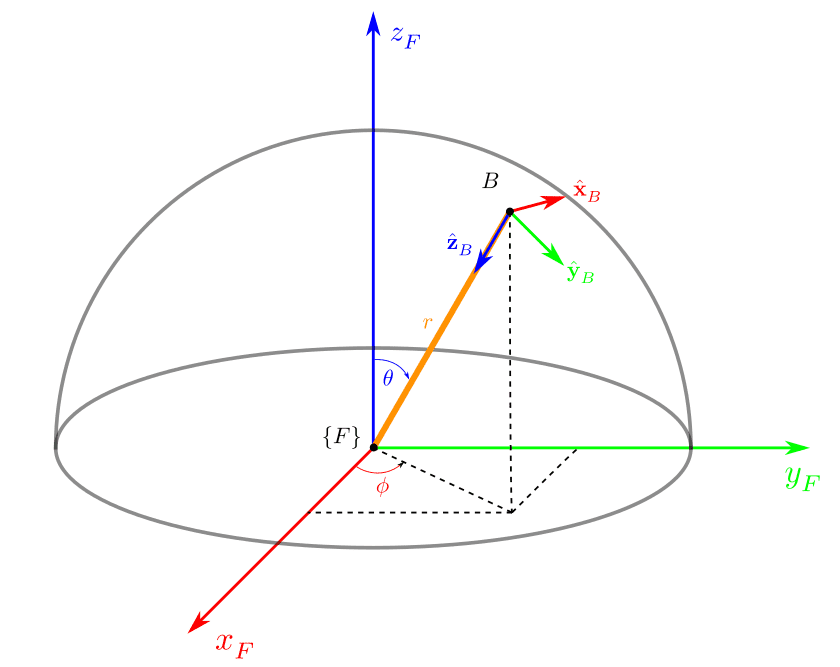
\includegraphics[width=12cm]{images/fulcrum-space.png}\\
\caption{Tool pose at target point $B$ calculated with respect to Fulcrum's reference frame $\lbrace F \rbrace$}
\end{figure}
\end{center}

The laparoscopic tool pose is given by the position and orientation vectors at target point $B$ with respect to the coordinate frame $\lbrace F \rbrace$.
The pose is given by the following transformation matrix
\[
{}^{F}T_B = \begin{bmatrix}
{}^{F}R_B & {}^{F}\mathbf{p}^{}_B \\
\mathbf{0} & 1 \\
\end{bmatrix}
\;\; where \;\;
{}^{F}R_B = \begin{bmatrix}
\hat{\mathbf{x}}^{}_B & \hat{\mathbf{y}}^{}_B & \hat{\mathbf{z}}^{}_B \\
\end{bmatrix}
\]

\[
\hat{\mathbf{x}}^{}_B = \hat{\mathbf{θ}} = cos(θ)cos(φ)\hat{\mathbf{x}}^{}_F + cos(θ)sin(φ)\hat{\mathbf{y}}^{}_F - sin(θ)\hat{\mathbf{z}}^{}_F
= \begin{bmatrix}
cos(θ)cos(φ) \\
cos(θ)sin(φ) \\
- sin(θ) \\
\end{bmatrix}
\]

\[
\hat{\mathbf{y}}^{}_B = \hat{\mathbf{φ}} = -sin(φ)\hat{\mathbf{x}}^{}_F + cos(φ)\hat{\mathbf{y}}^{}_F
= \begin{bmatrix}
-sin(φ) \\
cos(φ) \\
0 \\
\end{bmatrix}
\]

\[
\hat{\mathbf{z}}^{}_B = - \hat{\mathbf{r}} = - (sin(θ)cos(φ)\hat{\mathbf{x}}^{}_F + sin(θ)sin(φ)\hat{\mathbf{y}}^{}_F + cos(θ)\hat{\mathbf{z}}^{}_F)
= \begin{bmatrix}
-sin(θ)cos(φ) \\
-sin(θ)sin(φ) \\
-cos(θ) \\
\end{bmatrix}
\]

The position of the point $B$ is given in spherical coordinates by:
\begin{itemize}
	\item $r=ρ$ : outside penetration of laparoscopic tool
	\item $θ=β$ : altitude angle
	\item $φ=α$ : orientation angle
\end{itemize}
thus the position with respect to the coordinate frame $\lbrace F \rbrace$ is given by
\[
{}^{F}\mathbf{p}^{}_B = \begin{bmatrix}
ρsin(β)cos(α) \\
ρsin(β)sin(α) \\
ρcos(β) \\
\end{bmatrix} = ρ \hat{\mathbf{r}}
\]

The above goal point must be the same as the $TCP$ point of the robot's end-effector. This means, that this pose must be converted with respect to the robot's reference frames.
\[
{}^{U}T^{}_{TCP} = {}^{U}T^{}_{B}
\]
\[
{}^{U}T^{}_{0} \; {}^{0}T^{}_{7} \; {}^{7}T^{}_{TCP} = {}^{U}T^{}_{F} \; {}^{F}T^{}_{B}
\]
\begin{equation}
{}^{0}T^{}_{7} = {}^{U}T^{-1}_{0} \; {}^{U}T^{}_{F} \; {}^{F}T^{}_{B} \; {}^{7}T^{-1}_{TCP}
\end{equation}

\subsection{Pivoting motion with respect to Fulcrum Point}

\subsubsection{Circular trajectory of tool tip}

\begin{center}
\begin{figure}[H]
\centering
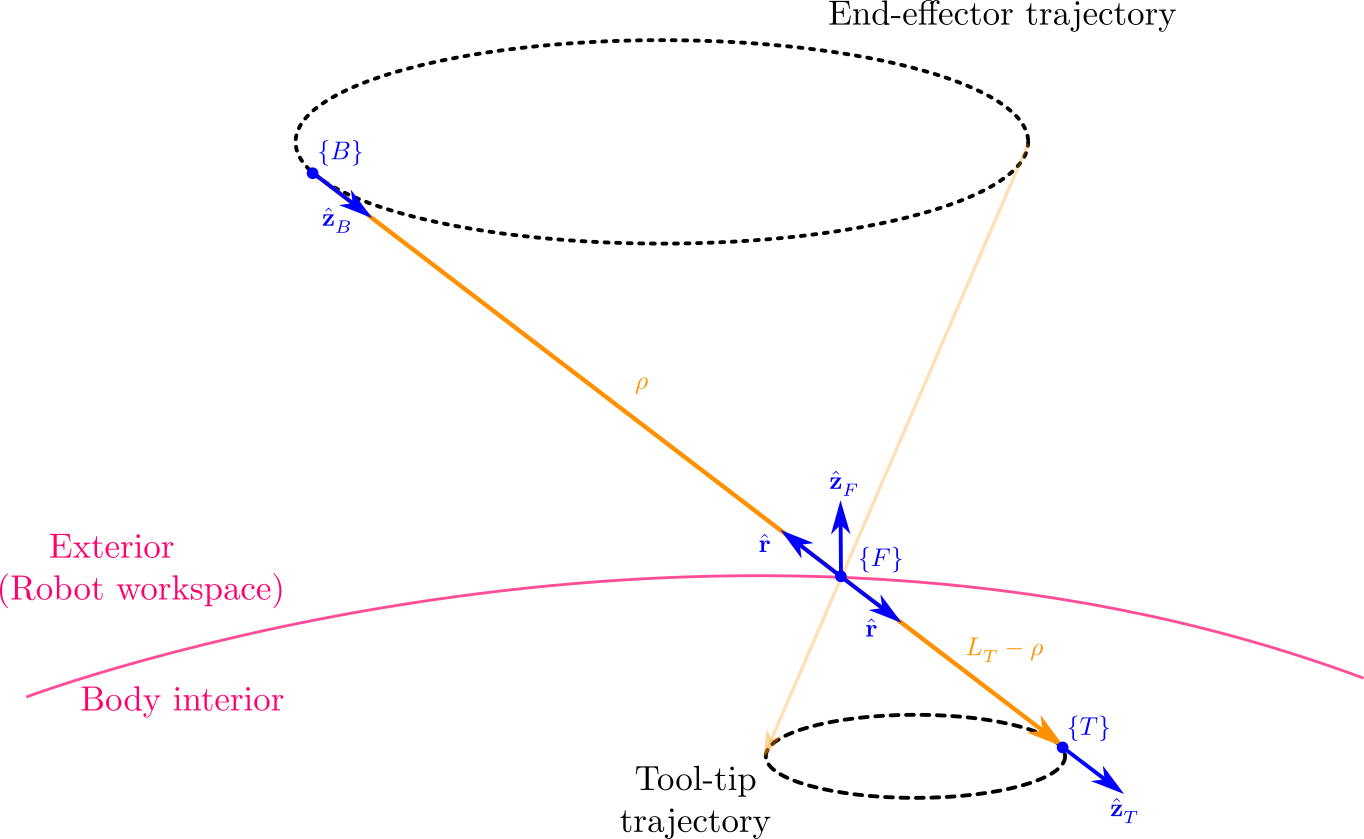
\includegraphics[width=12cm]{images/circular-trajectory-wrt-fulcrum.png}\\
\caption{Circular trajectory of tool tip with respect to Fulcrum reference frame}
\end{figure}
\end{center}


We first consider the motion of the laparoscopic tool tip on a circle parallel to a z-plane, with respect to the $\lbrace F \rbrace$ coordinate frame.
\[
(x^{}_{F} - x^{}_{F0})^2 + (y^{}_{F} - y^{}_{F0})^2 = r_0^2, \;\; z^{}_{F} = z^{}_{F0}
\]
It's often more convenient to express trajectories in a parametric form, which makes it easier to calculate all the waypoints of the trajectory
\[
\begin{cases}
x^{}_{F} = r_0cos(2πt) + x^{}_{F0} \\
y^{}_{F} = r_0sin(2πt) + y^{}_{F0} \\
z^{}_{F} = z^{}_{F0}
\end{cases} ,
\;\;
t \in [0, 1]
\]
After having calculated the cartesian coordinates we can calculate the spherical coordinates as follows
\begin{equation}
\label{eqns:cartesian-to-spherical}
\begin{cases}
r = \sqrt{x^{2}_{F} + y^{2}_{F} + z^{2}_{F}} \\
θ = atan2 \left( \sqrt{x^{2}_{F} + y^{2}_{F}}, z^{}_{F} \right) \\
φ = atan2(y^{}_{F}, x^{}_{F})
\end{cases}
\end{equation}


\subsubsection{Line segment trajectory of tool tip}

\begin{center}
\begin{figure}[H]
\centering
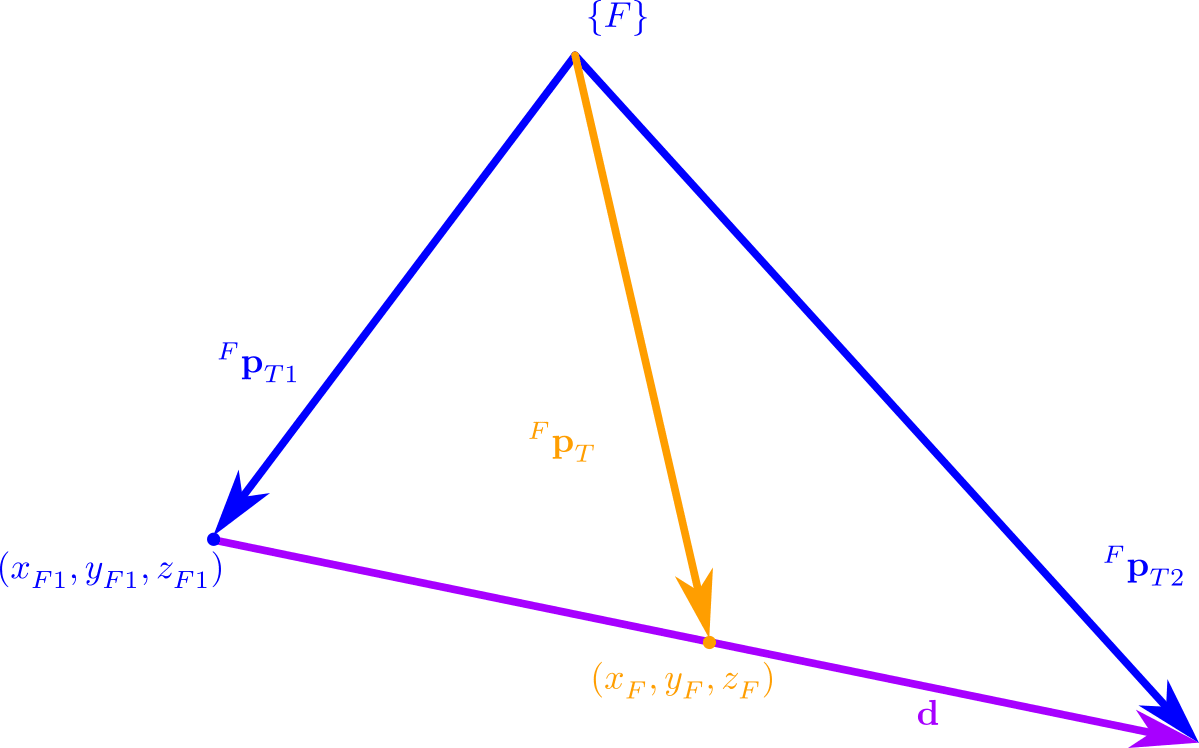
\includegraphics[width=10cm]{images/line-segment-trajectory-wrt-fulcrum.png}\\
\caption{Line segment trajectory of tool tip with respect to Fulcrum reference frame}
\end{figure}
\end{center}
\[
\mathbf{d} = {}^{F}\mathbf{p}^{}_{T2} - {}^{F}\mathbf{p}^{}_{T1} = [l, m, n]^\top
\]
\[
{}^{F}\mathbf{p}^{}_{T} = [x^{}_{F}, y^{}_{F}, z^{}_{F}]^\top
\]
\[
{}^{F}\mathbf{p}^{}_{T} = {}^{F}\mathbf{p}^{}_{T1} + t\mathbf{d}
\]
\[
t = \frac{x^{}_{F} - x^{}_{F1}}{l} = \frac{y^{}_{F} - y^{}_{F1}}{m} = \frac{z^{}_{F} - z^{}_{F1}}{n} \;\; t \in [0, 1]
\]
\[
\begin{cases}
x^{}_{F} = tl + x^{}_{F1} \\
y^{}_{F} = tm + y^{}_{F1} \\
z^{}_{F} = tn + z^{}_{F1}
\end{cases}
\]
After having calculated the cartesian coordinates we can calculate the spherical coordinates using the \ref{eqns:cartesian-to-spherical} equations.

\subsection{Task space analysis}

Dexterity analysis for tool's task space
\begin{equation}
\mathcal{D} = \mathcal{L}_q \mathcal{M}
\end{equation}
where
\begin{equation}
\mathcal{M} = \sqrt{det(J J^\top)}
\end{equation}
\begin{equation}
\mathcal{L}_{q}=1-\exp\left\{-\kappa\prod_{i=1}^{n_{k}}\frac{(q_{ {i}}-q_{i,\min})(q_{i,\max}-q_{i})}{(q_{i,\max}-q_{i,\min})^{2}}\right\}
\end{equation}

%\newpage
\section{Path Planning}

\subsection{Sampling methods}

The path planning algorithms that were mostly used in this thesis belong to the category of sampling methods


\subsubsection{RRT Algorithms}

The R\textbf{apidly-exploring Random Trees} algorithm is a sampling planning method that searches for an obstacle-free motion plan from an initial state $x_{init}$ to a set of goal states $\mathcal{X}_{goal}$. We refer to a set 
of goal states, because apart from the one desired goal state there can be other neighbor states that are within the allowed position and orientation tolerances.

\begin{algorithm}[H]
\SetAlgoLined
\ForEach{replanning attempt}{
	initialize vertices $V \leftarrow \lbrace x_{init} \rbrace$\;
	initialize edges $E \leftarrow \varnothing$\;
	initialize search tree $T \leftarrow (V,E)$\;
	\While{time \leq maxPlanningTime}{
		$x_{rand} \leftarrow$ getSampleStateFrom($\mathcal{X}$)\;
		$x_{nearest} \leftarrow$ getNearestNodeInTreeToState($T, x_{rand}$)\;
		$x_{new} \leftarrow$ findLocalPlanFromTo($x_{nearest}, x_{rand}$)\;
		\If{isPathCollisionFree($x_{nearest}, x_{rand}$)}{
			$V \leftarrow V \cup \lbrace x_{new} \rbrace $\;
			$E \leftarrow E \cup \lbrace (x_{nearest}, x_{rand}) \rbrace $\;
			\If{$x_{new} \in \mathcal{X}_{goal}$}{
				\Return SUCCESS and path plan $T=(V,E)$
			}
		}
	}
}
\Return FAILURE and $T=(V,E)$
\caption{RRT Algorithm}
\end{algorithm}

Other variations of the RRT Algorithm, which are also available in the OMPL library, included in the MoveIt library of ROS framework  are:
\begin{itemize}
	\item \textbf{BiTRRT} Transition-based RRT
	\item \textbf{BiTRRT} Bidirectional Transition-based RRT
	\item \textbf{RRT*}
	\item \textbf{RRTConnect} with is the default OMPL path planner in ROS
	\item \textbf{LBTRRT} Lower Bound Tree RRT
\end{itemize}


\subsubsection{PRM Algorithms}

The \textbf{Probabilistic Roadmap} (PRM) algorithm is a sampling planning method that constructs a roadmap representation of $\mathcal{C}_{free}$ \textbf{before searching} for a solution. After the roadmap is successfully built, then the algorithm searches 
for a solution using a traditional graph-based search algorithm. A very important aspect of this algorithm is how the sampling of the free configuration space will be done. The sampling is usually performed using a 
uniform distribution except from the regions close to objects where the sampling is more dense.

\begin{algorithm}[H]
\SetAlgoLined
initialize vertices $V \leftarrow \lbrace x_{init} \rbrace$\;
initialize edges $E \leftarrow \varnothing$\;
initialize roadmap graph $G \leftarrow (V,E)$\;
\For{$i = 1, \ldots , n$}{
	$x_{rand,i} \leftarrow$ getSampleStateFrom($\mathcal{X}$)\;
	$\mathcal{N}(x_{rand,i}) \leftarrow$ getKNearestNeighbors($G=(V,E), x_{rand,i}$)\;
	$V \leftarrow V \cup \lbrace x_{rand,i} \rbrace $\;
	\ForEach{$x \in \mathcal{N}(x_{rand,i})$}{
		\If{there is no edge between $x$ and $x_{rand,i}$}{
			\If{isPathCollisionFree($x_{nearest}, x_{rand,i}$)}{
				$E \leftarrow E \cup \lbrace (x_{rand,i}, x), (x, x_{rand,i}) \rbrace$
			}
		}
	}
}
\Return $G=(V,E)$
\caption{PRM roadmap construction (preprocessing phase)}
\end{algorithm}

Other variations of the PRM Algorithm, which are also available in the OMPL library, included in the MoveIt library of ROS framework  are:
\begin{itemize}
	\item \textbf{PRM*}
	\item \textbf{LazyPRM}
	\item \textbf{LazyPRM*}
\end{itemize}


\subsection{Pick and place algorithm}

% Help on using the algorithme package
% http://ftp.ntua.gr/mirror/ctan/macros/latex/contrib/algorithm2e/doc/algorithm2e.pdf 
\begin{algorithm}[H]
\SetAlgoLined
\ForEach{surgical tool}{
	\tcc{Plan the Pick pipeline}
	set grasp pose\;
	set pre-grasp approach\;
	set post-grasp retreat\;
	set posture of eef before grasp (open gripper)\;
	set posture of eef during grasp (closed gripper)\;
	\tcc{Plan the Place pipeline}
	set place location pose\;
	set pre-place approach\;
	set post-grasp retreat\;
	set posture of eef after placing object\;
	Plan pick and place paths\;
}
\caption{Pick and Place algorithm}
\end{algorithm}

If the pick and place algorithm targets small objects, such as cubes or spheres or other small convex objects then the path planning is straightforward. In the case where, the object to pick and place has at least one 
dimension that is bigger than the others like a rod or other long objects, such as the surgical tools, used in this thesis, then the path planning becomes more complicated, because of the almost certain collisions 
of the tool with the links of the rest of the robot (the link of the end-effector will probably not collide with the tool).

%\newpage
\section{Trajectory Planning}

At this step, given the points of the desired path, a more detailed trajectory is calculated, 
which will contain all the waypoints that the robot will have to visit.

\subsection{Trajectory planning in cartesian coordinates}

Connect the points from path planning with line segments and add more points if needed

\begin{center}
\begin{figure}[H]
\centering
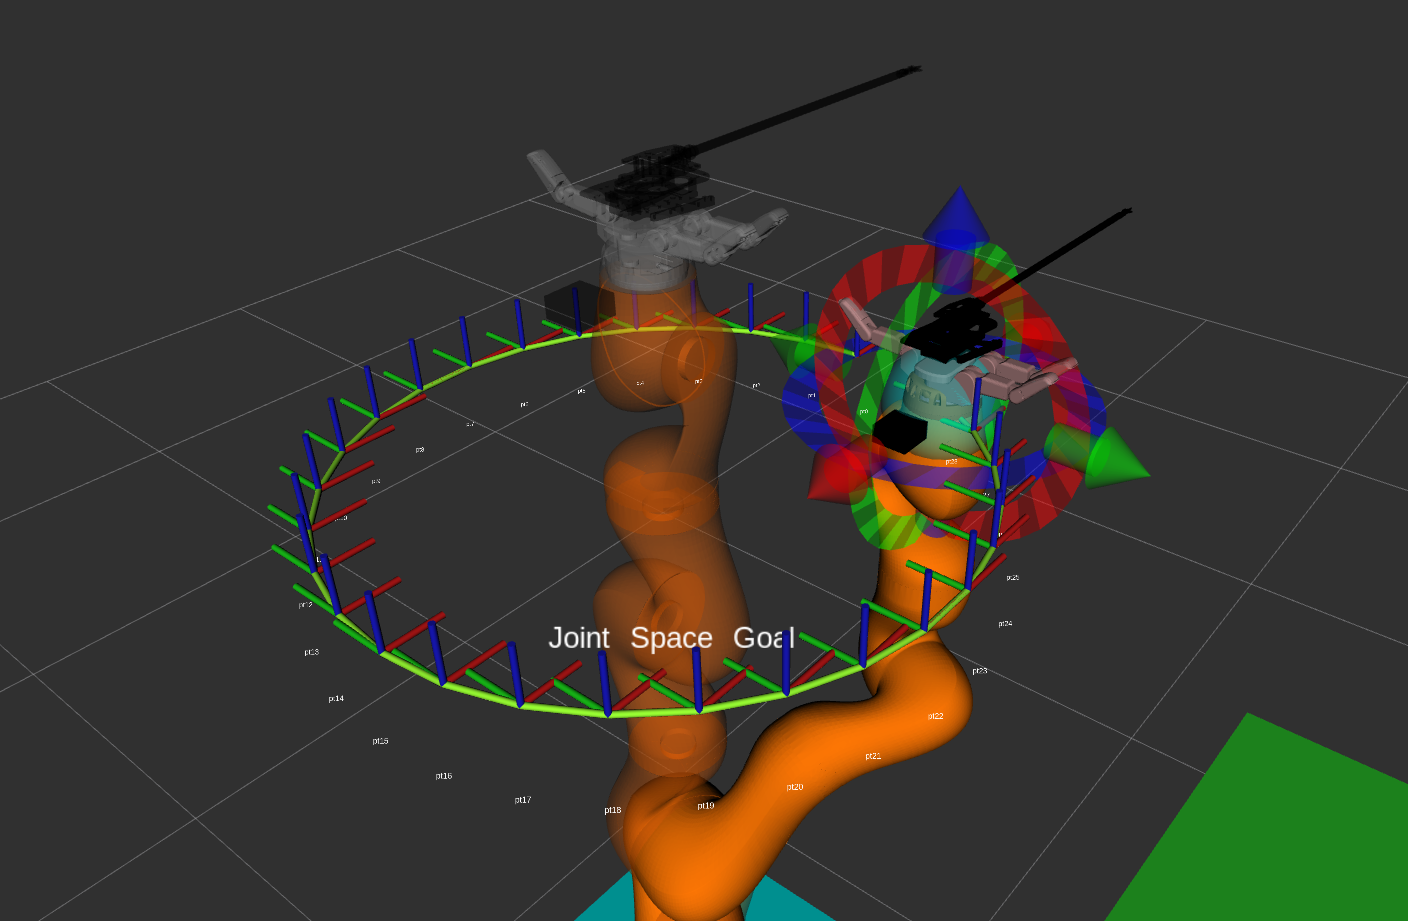
\includegraphics[width=0.7\textwidth]{images/simple_circular_traj1.png}\\
\caption{Circlular trajectory around the z axis of the home position of the robot}
\label{fig:circ-traj-out-of-angle-range}
\end{figure}
\end{center}

It is very important that the designed trajectory respects the joints angles' range. For example
depending on the starting position of the circular trajectory depicted at figure 
\ref{fig:circ-traj-out-of-angle-range}, the robot arm may reach it's joint bounds and in order to 
continue executing the trajectory it will have to make a sudden jump to reset the angles. 
This could have serious side-effects for both the surgical task and thus the patient, as well as 
for the operating staff, who control the robot.

\subsection{Trajectory planning in joint angles space}

\begin{center}
\begin{figure}[H]
\centering
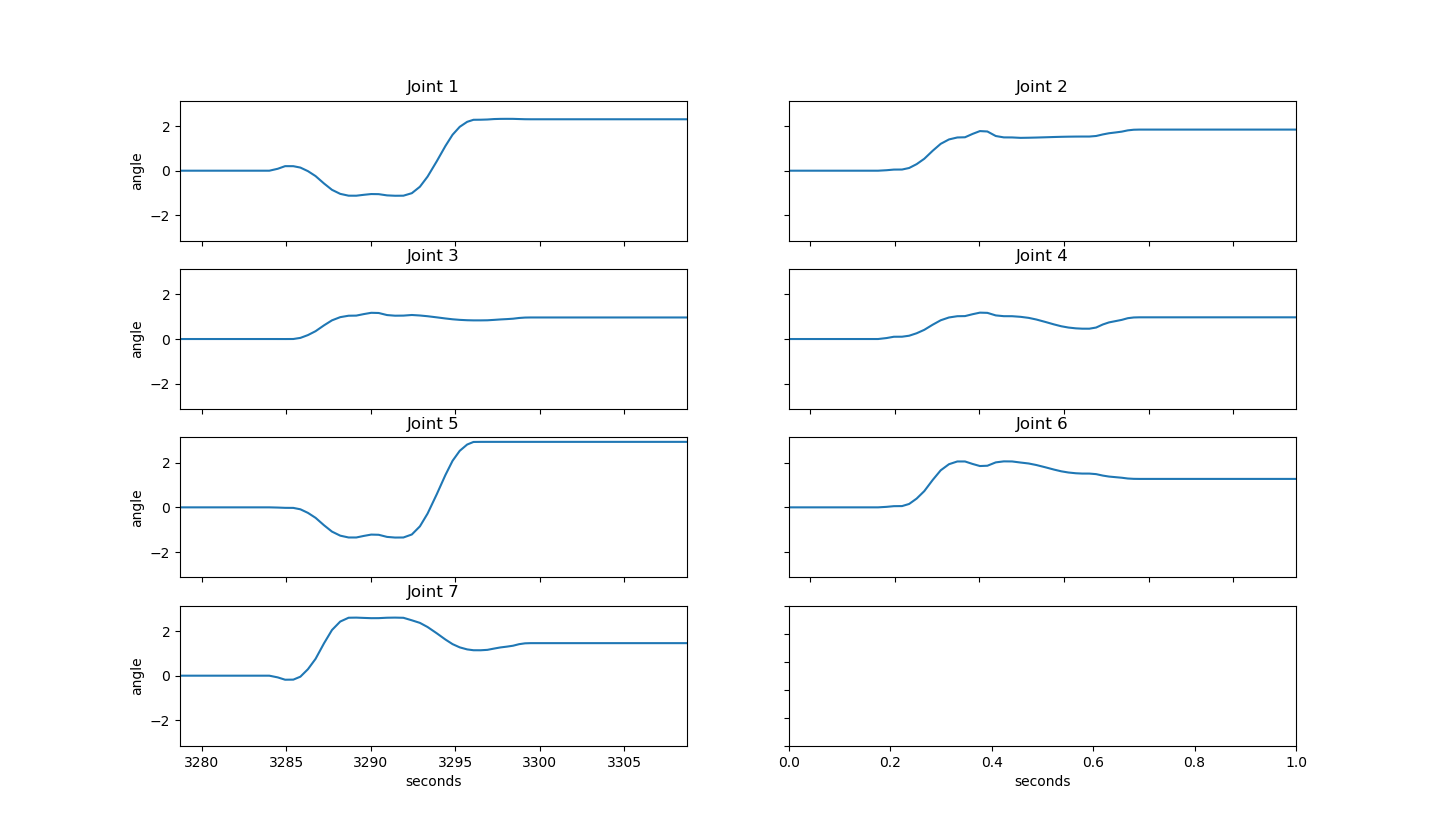
\includegraphics[width=\textwidth]{images/trajectory1-test1.png}\\
\caption{Trajectory diagrams in joints space.}
\end{figure}
\end{center}

%\newpage
\section{Simulation with the ROS framework}

\subsection{Gazebo simulation environment}

\begin{center}
\begin{figure}[H]
\centering
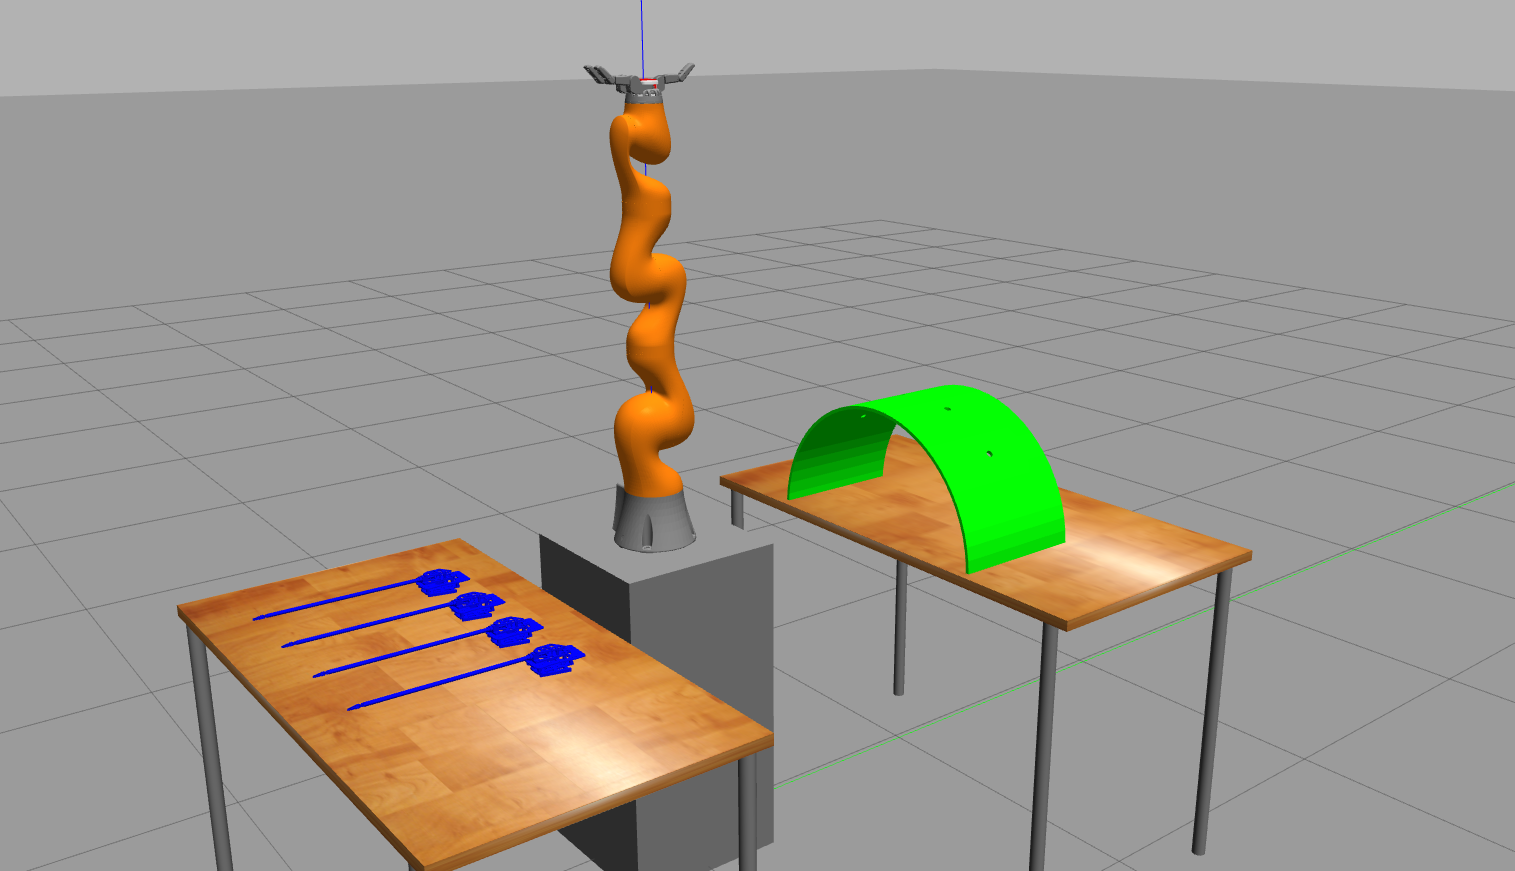
\includegraphics[width=12cm]{images/gazebo-sim1.png}\\
\caption{Simulation environment in Gazebo}
\end{figure}
\end{center}

\subsection{Visualization and Motion Planning with RViz and Moveit}

Motion Planning parameters outside of body:
\begin{itemize}
	\item Position tolerance: 50μm
	\item Orientation tolerance: 0.00005 deg
	\item Planning time: 10s
\end{itemize}

Motion Planning parameters inside of body:
\begin{itemize}
	\item Position tolerance:
	\item Orientation tolerance:
	\item Planning time
	\item End-effector interpolation step: 1mm
	\item Maximum velocity scaling factor
\end{itemize}


%----------------------------------------------------------------------------------------
%	BIBLIOGRAPHY, REFERENCES, TABLES
%----------------------------------------------------------------------------------------
\newpage
\nomenclature{$^{i-1}T_{i}$}{Transformation matrix from coordinate frame $\lbrace i \rbrace$ to coordinate frame $\lbrace i-1 \rbrace$ }
\nomenclature{$c_{i}$}{Shorthand notation for $cosθ_{i}$}
\nomenclature{$s_{i}$}{Shorthand notation for $sinθ_{i}$}
\nomenclature{$^{i-1}R_{i}$}{Rotation matrix from coordinate frame $\lbrace i \rbrace$ to coordinate frame $\lbrace i-1 \rbrace$ }
\nomenclature{$^{i-1}\mathbf{p}_{iO}$}{Position vector from the origin of the coordinate frame $\lbrace i \rbrace$ to the origin of the coordinate frame $\lbrace i-1 \rbrace$ }
\nomenclature{$J^{\dagger}$}{Pseudoinverse of the Jacobian}
\nomenclature{$\mathcal{M}$}{Manipulability measure of the robotic arm}
\nomenclature{$\mathcal{L}_q$}{Dexterity measure of the robotic arm}
\nomenclature{$\hat{\mathbf{x}},\hat{\mathbf{y}},\hat{\mathbf{z}}$}{Unit vectors of $x,y,z$ axes respectively }
\nomenclature{$\hat{\mathbf{r}},\hat{\bm{\theta}},\hat{\bm{\phi}}$}{Unit vectors of $r,θ,φ$ axes respectively, in spherical coordinates }
\nomenclature{$\theta, \phi, \psi$}{roll, pitch, yaw angles, also known as the Euler angles}
\nomenclature{$\mathcal{C}$}{Configuration Space}
\nomenclature{$\mathcal{C}_{obs}$}{Obstacle Space}
\nomenclature{$\mathcal{C}_{free}$}{Free Configuration Space}
\nomenclature{$q_i$}{Angle position of joint $i$}
\nomenclature{$\dot{q}_i$}{Angle velocity of joint $i$}
\nomenclature{$\mathbf{q}$}{Angle positions vector of all joints}
\nomenclature{$\ddot{q}_i$}{Angle acceleration of joint $i$}
\nomenclature{$\dddot{q}_i$}{Angle jerk of joint $i$}
\nomenclature{$τ$}{Time constant, represents a specific time duration in a trajectory velocity profile or in a system controller}
\nomenclature{RCM}{Remote Center of Motion}
\nomenclature{TCP}{Tool's Center Point}
\nomenclature{$\mathbf{C}$}{Covariance matrix}
\nomenclature{$\mathbb{R}^n$}{Vector space of n-dimensional real-valued vectors}
\nomenclature{$\mathbb{R}^{n \times m}$}{Vector space of all real-valued $n \times m$ matrices}
\nomenclature{$SE(3)$}{Special Euclidean Group. Vector space of all 3D transformations}
\nomenclature{$SO(3)$}{Special Orthogonal Group. Vector space of all 3D rotations}
\nomenclature{$\mathbb{H}$}{Quaternions group. A four-dimenional space with basis $\mathbf{1},\mathbf{i},\mathbf{j},\mathbf{k}$ that includes all quaternions. In the context of this thesis quaternions are used for 3D rotations instead of matrices from $SO(3)$}
\nomenclature{$\mathbb{S}$}{Surgical 3D taskspace}
\nomenclature{$\mathbb{P}$}{Pivot paths 3D taskspace, $\mathbb{P} \subset \mathbb{T}$}
\nomenclature{$\mathbb{T}$}{Robot's Euclidean 3D taskspace}
\nomenclature{$\mathbb{J}$}{Joint taskspace}
\printnomenclature

%\newpage
\cleardoublepage
\phantomsection
\addcontentsline{toc}{section}{\listfigurename}
\listoffigures

%\newpage
%\cleardoublepage
\phantomsection
\renewcommand{\listoflistingscaption}{List of programs}
\addcontentsline{toc}{section}{\listoflistingscaption}
\listoflistings

%\newpage
\nocite{*}
\printbibliography[heading=bibintoc,title={Bibliography}]

%\end{otherlanguage}
\end{document}
